\documentclass[a4paper,12pt]{report}

% Page layout
\usepackage[left=3cm,right=2cm,top=2.5cm,bottom=2.5cm]{geometry}

% Figures
\usepackage[margin=\the\parindent,small,bf,rm]{caption}
\usepackage{graphicx}
\usepackage{pdfpages}
\setlength{\abovecaptionskip}{7.5pt}  % spacing above and below captions

% Font and text
\usepackage[afrikaans,english]{babel}
\usepackage{microtype}
\usepackage{setspace}
\usepackage[normalem]{ulem}
\newcommand{\myemph}[1]{{\rmfamily\bfseries#1}}
\sloppy
\onehalfspacing

% Headings
\usepackage[raggedright,rm,bf]{titlesec}
\titlelabel{\thetitle.\ }
\titleformat{\chapter}[hang]{\huge\bfseries\rmfamily}{\thechapter}{0.5em}{\Huge \raggedright}
% \titleformat{\chapter}[display]{\centering\huge\bfseries\sffamily}{\chaptertitlename\ \thechapter:}{15pt}{}
\titlespacing*{\chapter}{0pt}{0pt}{40pt}  % remove spacing before chapter headings

% Table of contents
\makeatletter
\let\originall@chapter\l@chapter
\def\l@chapter#1#2{\originall@chapter{{\rmfamily #1}}{#2}}
\makeatother
\let \savenumberline \numberline
\def \numberline#1{\savenumberline{#1.}}

% Mathematics
\usepackage[cmex10]{amsmath}
\usepackage{amssymb, mathrsfs}
\usepackage{cancel}
\DeclareMathOperator*{\argmax}{arg\,max}
\newcommand{\T}{^\textrm{T}}
\newcommand{\tr}{\textrm{tr}}
\renewcommand{\vec}[1]{\boldsymbol{\mathbf{#1}}}
\newcommand{\defeq}{\triangleq}

% Tables
\usepackage{booktabs}
\usepackage{tabularx}
\usepackage{multirow}
\newcommand{\mytable}{
    \centering
    \small
%     \renewcommand{\arraystretch}{1.2}
    \renewcommand{\arraystretch}{1.2}
    }
\renewcommand{\tabularxcolumn}[1]{m{#1}}
\newcolumntype{C}{>{\centering\arraybackslash}X}
\newcolumntype{L}{>{\raggedright\arraybackslash}X}

% Header and footer
\usepackage{fancyhdr}
\pagestyle{fancy}
\fancyhf{}
\renewcommand{\sectionmark}[1]{\markright{\normalsize \thesection.\ #1}}
\fancyhead[C]{\nouppercase{\textit{\rightmark}}}
\fancyhead[RO]{\thepage}  % printing (keep this)
% \fancyhead[LE]{\thepage}  % printing (keep this)
\fancyfoot{}
\setlength\headheight{14.5pt}
\renewcommand{\headrulewidth}{0pt}
\fancypagestyle{plain}{\fancyhead{}
                       \renewcommand{\headrulewidth}{0pt}
                       \fancyfoot[C]{\thepage}}

% Pseudo-code
\usepackage{algorithm}  % should go before \usepackage{hyperref}

% Table of contents and hyperlinks
\usepackage{hyperref}
\hypersetup{colorlinks=true,linktoc=all,citecolor=black,linkcolor=black}
\usepackage[nottoc]{tocbibind}

% Pseudo-code
\usepackage{algpseudocode}  % should go after \usepackage{hyperref}
\renewcommand{\thealgorithm}{\arabic{chapter}.\arabic{algorithm}} 
\captionsetup[algorithm]{labelfont={bf,rm},font=small,labelsep=colon}

% Bibliography
\usepackage{cite}  % automatically reorder inline citations
\bibliographystyle{IEEEtran}

% Fix titlesec issue
\usepackage{etoolbox}
\makeatletter
\patchcmd{\ttlh@hang}{\parindent\z@}{\parindent\z@\leavevmode}{}{}
\patchcmd{\ttlh@hang}{\noindent}{}{}{}
\makeatother


\begin{document}

% Front matter
\graphicspath{{frontmatter/fig/}}
\pagenumbering{Alph}

\begin{titlepage}
\begin{center}


\includegraphics[width=10cm]{USlogo-top}

\vfill

{\rmfamily \bfseries \huge Using computer vision to process speech \par}

\vfill

{\large {\Large Marthinus Bosman} \\ 18955185 \par}

\vfill

\vfill

{Report submitted in partial fulfilment of the requirements of the module \\
Project (E) 448 for the degree Baccalaureus in Engineering in the Department of
Electrical and Electronic Engineering at Stellenbosch University. \par}

\vfill

{\large {Supervisor}: Dr H. Kamper} %\\
% Department of Electrical and Electronic Engineering \par}

\vfill

{\Large October 2018}
\end{center}
\end{titlepage}

\pagenumbering{roman}
\chapter*{Acknowledgements}
% \addcontentsline{toc}{chapter}{Acknowledgements}
\makeatletter\@mkboth{}{Acknowledgements}\makeatother

I would like to thank the following:

\begin{itemize}
\item My supervisor, Dr
Herman Kamper, for continuously supporting me throughout this process and his eagerness to help wherever possible.
Also for supplying useful code to complete some of the tasks within this report.
\item My Parents, Deon and Marijke Bosman, for your continued love and support, without which I would never have made it to this point.
\item My girlfriend, Marizanne Visagie, for working alongside me and keeping me company until early in the morning all those weekends.
\item The Electrical and Electronic Engineering group of 2018, for their fantastic team mentality throughout this degree, always working together to solve problems and never leaving anyone behind.
\item Google and their Google Cloud Platform for their free trial period and Datalab loophole to use more CPUs than allowed, without which the total processing time for this project would have taken more than 16\,000 hours to complete. 
\end{itemize}
\makeatletter
\newcommand{\unchapter}[1]{%
	\begingroup
	\let\@makeschapterhead\@gobble % make \@makechapterhead do nothing
	\chapter*{#1}
	\endgroup
}
\makeatother

\unchapter{Declaration}
\begin{center}

\includegraphics[width=10cm]{USlogo-top}
\addcontentsline{toc}{chapter}{Declaration}
\makeatletter\@mkboth{}{Declaration}\makeatother
\\
{\rmfamily \bfseries \large Plagiaatverklaring / \textit{Plagiarism Declaration} \par}

\begin{enumerate}
	\item Plagiaat is die oorneem en gebruik van die idees, materiaal en ander intellektuele
	eiendom van ander persone asof dit jou eie werk is.\\
	\textit{Plagiarism is the use of ideas, material and other intellectual property of another’s work
	and to present is as my own.}
	
	\item Ek erken dat die pleeg van plagiaat 'n strafbare oortreding is aangesien dit ‘n vorm van
	diefstal is.\\
	\textit{I agree that plagiarism is a punishable offence because it constitutes theft.}
	
	\item Ek verstaan ook dat direkte vertalings plagiaat is.\\
	\textit{I also understand that direct translations are plagiarism.}
	
	\item Dienooreenkomstig is alle aanhalings en bydraes vanuit enige bron (ingesluit die
	internet) volledig verwys (erken). Ek erken dat die woordelikse aanhaal van teks
	sonder aanhalingstekens (selfs al word die bron volledig erken) plagiaat is.\\
	\textit{Accordingly all quotations and contributions from any source whatsoever (including the
	internet) have been cited fully. I understand that the reproduction of text without
	quotation marks (even when the source is cited) is plagiarism.}
	
	\item Ek verklaar dat die werk in hierdie skryfstuk vervat, behalwe waar anders aangedui, my
	eie oorspronklike werk is en dat ek dit nie vantevore in die geheel of gedeeltelik
	ingehandig het vir bepunting in hierdie module/werkstuk of ‘n ander module/werkstuk
	nie.\\
	\textit{I declare that the work contained in this assignment, except where otherwise stated, is
	my original work and that I have not previously (in its entirety or in part) submitted it for
	grading in this module/assignment or another module/assignment.}
\end{enumerate}

\begin{table}
\begin{tabular} { | p{9.1cm} | p{6cm} | }
	\hline
	& \\
	& \\
	 \textbf{ Studentenommer / \textit{Student number}} & \textbf{ Handtekening / \textit{Signature}} \\
	\hline
	& \\
	& \\
	\textbf{ Voorletters en van / \textit{Initials and surname }} & \textbf{ Datum / \textit{Date}} \\
	\hline
\end{tabular}
\end{table}

\end{center}
\chapter*{Abstract}
\addcontentsline{toc}{chapter}{Abstract}
\makeatletter\@mkboth{}{Abstract}\makeatother

\subsubsection*{English}

One of the fundamental difficulties in speech recognition is the task of extracting useful features from the highly variable time domain signal due to different speakers, tones, channels and acoustic conditions.
In most state-of-the-art computer vision systems, convolutional neural networks (CNNs) are used to automatically learn how to extract relevant features.
In this study, we aim to evaluate how general these features are.
Specifically, we evaluate the features extracted from a trained vision CNN on speech spectrograms against existing techniques such as filter banks and Mel-frequency Cepstral Coefficients (MFCCs).
The features were evaluated against each other using dynamic time warping to achieve an average precision score per feature.
We achieved an average precision (AP) score of X, improving feature extraction significantly from both existing methods.
Furthermore, we present some insight into the features extracted by the model as well as a new technique for High-throughput computing using Google Cloud Platform.

\selectlanguage{afrikaans}

\subsubsection*{Afrikaans}

Een van die fundamentele probleme in spraakherkenning is om nuttige eienskappe vanuit die hoogs veranderlike klankgolf te onttrek weens verskillende sprekers, toonhoogtes, kanale en akoestiese toestande.
In meeste moderne rekenaarvisie netwerke word konvolusionele neurale netwerke (kNN) gebruik om automaties te leer hoe om relevante eienskappe te onttrek.
In hierdie studie beoog ons om te evalueer hoe algemeen hierdie kenmerke is.
Ons evalueer spesifiek die eienskappe wat deur 'n opgeleide visie kNN op spraakspektrogramme verkry is teen bestaande tegnieke soos filterbanke en Melfrekwensie Cepstral Koëffisiënte.
Die eienskappe was evalueer teen mekaar deur dinamiese tydverduistering te gebruik om 'n algemene akkuraatheid punt te behaal.
Die top kNN eienskappe het 'n algemene akkuraatheidspunt van X behaal, wat 'n verbetering is op beide bestaande metodes.
Verder bied ons ook insig in die eienskappe wat deur die model verkry word sowel as 'n nuwe tegniek vir Hoë-deursettingsberekening deur gebruik te maak van Google Cloud Platform.

\selectlanguage{english}
\tableofcontents
\listoffigures
\listoftables
\chapter*{Nomenclature\markboth{}{Nomenclature}}
\addcontentsline{toc}{chapter}{Nomenclature}

% \vspace*{-3mm}
\subsubsection*{Variables and Functions}

\begingroup
\renewcommand{\arraystretch}{1.2}
\renewcommand{\tabularxcolumn}[1]{p{#1}}
\begin{tabularx}{\textwidth}{@{}p{2.5cm}L}
$	O()	$&	The order of a function in terms of the number of input elements.	\\
$	\mathtt{DTW}()	$&	The Dynamic Time Warping function.	\\
$	\mathcal{F} \{\}	$&	The Fourier Transform function.	\\
$	H[k]	$&	The Discrete Fourier Transform of the function $h[k]$.	\\
$	w[n]	$&	The discrete Hamming Window function.	\\
$	f_s	$&	Sampling Frequency.	\\
$	H_m(k)	$&	The function to obtain triangular filters on the Mel-scale.	\\
$	\mathtt{DCT}()	$&	The Discrete Cosine Transform function.	\\
$	d_t	$&	The delta coefficients at index $t$.	\\
$	w_j	$&	The weight assigned to neuron $j$ within a neural network.	\\
$	b_j	$&	The bias assigned to neuron $j$ within a neural network.	\\
$	\mathrm{max}(a, b)	$&	Returns the largest value between $a$ and $b$.	\\
$	\mathtt{d}(\underline{a}, \underline{b})	$&	The cosine distance between vectors $\underline{a}$ and $\underline{b}$.	\\
$	{||\underline{x}||}_2	$&	The L2-norm of vector $\underline{x}$.	\\
$	N	$&	The total amount of frames, window size or number of items, depending on the context.	\\

\end{tabularx}
\endgroup


\newpage
\subsubsection*{Acronyms and Abbreviations}

\begingroup
\renewcommand{\arraystretch}{1.2}
\begin{tabular}{@{}p{2.5cm} l}
    AP	 &	Average Precision	\\
    API	 &	Application Programming Interface	\\
    CNN	 &	Convolutional Neural Network	\\
    CPU	 &	Central Processing Unit	\\
    DCT	 &	Discrete Cosine Transform	\\
    DFT	 &	Discrete Fourier Transform	\\
    DTW	 &	Dynamic Time Warping	\\
    FFT	 &	Fast Fourier Transform	\\
    FT	 &	Fourier Transform	\\
    GB	 &	Gigabyte	\\
    GCE	 &	Google Compute Engine	\\
    GCP	 &	Google Cloud Platform	\\
    GCS	 &	Google Cloud Storage	\\
    kB	 &	Kilobyte	\\
    LPF	 &	Low-Pass Filter	\\
    MFCC &	Mel-Frequency Cepstral Coefficients	\\
    OH	 &	Ohio	\\
    OS	 &	Operating System	\\
    ReLU &  Rectified Linear Unit \\
    RGB	 &	Red Green Blue	\\
    SaaS &	Software as a Service	\\
    STFT &	Short Time Fourier Transform	\\
    vCPU &	virtual Central Processing Unit	\\
    VM	 &	Virtual Machine	\\
    WAV	 &	Waveform Audio File Format	\\
\end{tabular}
\endgroup

\newpage
\pagenumbering{arabic}

% Contents
\graphicspath{{introduction/fig/}}

\chapter{Introduction}
\label{chap:introduction}

Modern deep neural networks achieve unparalleled accuracy scores on many machine learning task.
Although this feat is remarkable, the vast amounts of processing power and labelled training data necessary to achieve these levels of accuracy greatly limit the amount of problems they can be applied to.
Making these trained models applicable to different types of tasks could massively increase their possible uses without the need for excessive training on each different task.
But could the learned features of these networks be applied to different tasks?

When humans are born, our brains are bombarded immediately and continuously with data of all different formats about the world around us, such as visual, auditory, taste, smell, touch, etc.
To process each of these data streams individually would take an enormous amount of processing power.
Instead, using shared processing techniques for different sensory input could lower the needed processing power significantly, and recent studies have shown that direct relationships between the visual cortex and primary auditory cortex exist\cite{doi:10.1002/hbm.20560}, suggesting that this technique might well be the case within the human brain.

With modern neural networks being loosely inspired by the brains' structure, it may therefore stand to reason that using the same processing techniques employed by the brain in neural networks could show meaningful results.
Thus, we can attempt to leverage the neural networks for one data type to reveal useful results when applied to another. 

We focus on the task of evaluating feature extraction techniques from a trained vision neural network when applied to speech data against existing feature extraction techniques.
Our goal is to achieve a feature set that better represents speech data for the task of speech recognition, and to find some qualitative insight on why these extracted features are more useful. 

\section{Motivations}

The task of image classification has improved greatly in the past decades, with models such as the VGG16 network \cite{DBLP:journals/corr/SimonyanZ14a} achieving an accuracy score of 92.7\% on the ImageNet database in 2014, and newer models achieving ~98\% accuracy scores.\cite{ILSVRC15} A large contributor to these results is the amount of training data available to these models, with the ImageNet database consisting of over 14 million labelled images.

The task of speech recognition for the English language has seen similar strides in accuracy growth over the years, but for roughly 4600 languages spoken by more than 1000 people throughout the world and 11 official languages in South Africa, the task of speech recognition is far from solved.
The limited amount of labelled speech data on all these languages greatly limit the effectiveness of neural networks.
The task of acquiring speech data for different languages and then labelling it is expensive and time consuming.
Speech data also varies widely due to different speakers, tones, channels and acoustic conditions.
It is thus of utmost importance that the features extracted from the data be as efficient as possible to lower the training needs of models.

\section{Methodology}

Image classification made a significant breakthrough in accuracy in 2014 when convolutional neural networks were used to extract features from images through convolutional filters.
These networks learn from data and adapt the filters to automatically extract the most useful features.
We aim to test the general nature of these convolutional filters by applying them to speech spectrograms.

The VGG16 CNN trained on the ImageNet database has 13 layers of filters, each with between 64 and 512 filter kernels.
We adapted the VGG16 network to run be able to run on differently sized spectrograms and filterbanks as well as get the output of individual convolutional layers and kernels.
We then ran the first 8 layers of filters on speech spectrograms and filterbanks generated from spoken words in the Buckeye English Corpus to obtain feature sets for each word.
This resulted in 1152 feature sets for each word, and 3\,148\,416 features in total.

The quality of each of these features were determined by using dynamic time warping to calculate a distance metric between the same feature set for two words \cite{DBLP:conf/interspeech/CarlinTJH11}. If this distance score better distinguishes two different words from two similar words for a given feature set, that feature set then more accurately describes the speech data.
Thus, for a given feature set, the features for each word was compared to every other word, and the distance scores between them were stored in two arrays, one for scores between the same word and one for different words.
For each feature set, these distance scores were used to calculate an average precision score, which indicates the separability of the two arrays and thus the efficacy of the given feature set.
These scores were then evaluated against average precision scores for generic filterbanks, MFCCs and spectrograms.

The feature sets with the top 5 highest average precision were combined to form a single feature set, and the average precision for that feature set was calculated.
This resulted in a feature set with an average precision  higher than any generic feature extraction technique.

\section{Contributions}

This study makes several contributions towards the task of feature extraction for speech data.
Specifically, we make the following contributions:

\begin{itemize}
\item We provide a method of feature extraction on speech data that outperforms filterbanks and MFCCs as a method of preprocessing for speech recognition.
With this technique, we hope to allow training of speech recognition models using less speech data.
\item We explore new insight into using visual processing techniques on speech spectrograms as a means of extracting useful information from the speech data, qualitatively analysing the visual properties obtained from the top performing convolutional filters.
\item We make available a library of 2304 different speech feature sets from 2733 different spoken words extracted from the Buckeye Corpus, as well as open-source examples on how to generate these features.
\item We develop a new technique for High-throughput Computing using GCP's Cloud Functions in conjunction with GCE instances.
\item We developed and made available a code base for extracting features from speech data using the newly developed technique, as well as an adapted VGG16 TensorFlow model with functionality to allow extraction and visualisation of the outputs of individual convolutional layers and filter kernels applied to differently sized  images.
\end{itemize}
\chapter{Existing Techniques and Models}

In this study we aim to improve on existing speech feature extraction using a trained vision CNN.
In order to understand this process, we first need to understand the feature extraction techniques as well as how CNNs work.
This chapter provides an overview of each speech feature extraction technique, namely spectrograms, filterbanks and MFCCs, and the convolution process within convolutional neural networks. 
Thereafter it looks specifically at the inner structure of the VGG16 vision network.

\section{Speech Features}

For the task of speech recognition, generic time domain sound waves are an ineffective choice for input data. 
They are large files that would cause the resultant machine learning model to have to accept massively large input sizes. 
For this reason, the sound waves are often converted to the frequency domain into spectrograms. 

Spectrograms contain all the useful information about the speech data in a far more concise format, but can sometimes still be fairly large data structures. 
Therefore, spectrograms are usually further reduced to filterbanks and MFCCs, which more accurately reflect the way humans perceive audio information and also further reduce the input data dimensions and size.

\subsection{Spectrograms}

Speech data is often very inefficient to work with in the time domain, therefore, discrete time domain signals are often converted to the frequency domain via a process called Discrete Fourier Transform (DFT). 
The DFT ($H[k]$) of a discrete time domain signal ($h[n]$) is calculated by first by first windowing the signal using the Hamming Window ($w[n]$) with window size $N$ to obtain $h_{w}[t]$:

\begin{equation}
    w[n] = 0.54+0.46\cos\Big(\frac{\pi n}{N-1}\Big), \quad 0 \leq n \leq N-1
\end{equation}

\begin{equation}
    h_{w}[n] = h_{s}[n] \cdot w[n]
\end{equation}

Thereafter, the signal must be made periodic in time in order to discretise the frequency domain signal. 
This is done by convolving the signal with the a periodic impulse function in $N$ to obtain $h_{p}[n]$:

\begin{equation}
    h_{p}[n] = h_{w}[n] \ast \delta(n-kN), \quad k=(0,1,\dotsc,N-1)
\end{equation}

The FT of $h_{p}[n]$ then forms our desired DFT function:

\begin{equation}
    H[k] = \mathcal{F} \{ h_{p}[n] \}
\end{equation}

In summary, this process can be written as follows:

\begin{equation}
    H[k] = \mathtt{DFT} \{ h_{p}[n] \} = \displaystyle\sum_{n=0}^{N-1} h[n] \cdot e^{\displaystyle\frac{-j2\pi kn}{N}}
\end{equation}

The problem with simply calculating the DFT of speech data, is that speech is a non-stationary signal, Thus the DFT will calculate each frequency present throughout the entire word. 
Therefore, spectrograms are obtained performing Short Time Fourier Transform (STFT) on the speech sound wave. 

STFT works by segmenting the sound wave into frames of length $N$, separated by length $R$, and then calculating the log power of the DFT for each individual frame and concatenating the 2-dimensional functions into a 3-dimensional surface. 
The third-dimension is then converted to colour, forming a spectrogram of the sound signal. 
This process is visualised in Figure~\ref{fig:spec_example} for the function $h[t]=\sin\big(2\pi f_{w_1} t + 100 \cdot \cos(2\pi f_{w_2} t) \big)$, with $f_{w_1}= 8 \mathrm{kHz}$, $f_{w_2}= 4 \mathrm{Hz}$.
The power of the DFT can be calculated as follows:

\begin{equation}
    P = \log\bigg(\frac{|\mathtt{DFT}(x_i)|^2}{N}\bigg)
\end{equation}

It is important to note that, computationally, the DFT is calculated by means of the FFT function, which gives the exact same results, but exploits the symmetries and periodicity of the DFT to save on computation. 
The FFT changes the DFT from an $O(N^2)$ computation to $O(N)$.

\begin{figure}[h]
    \centering
    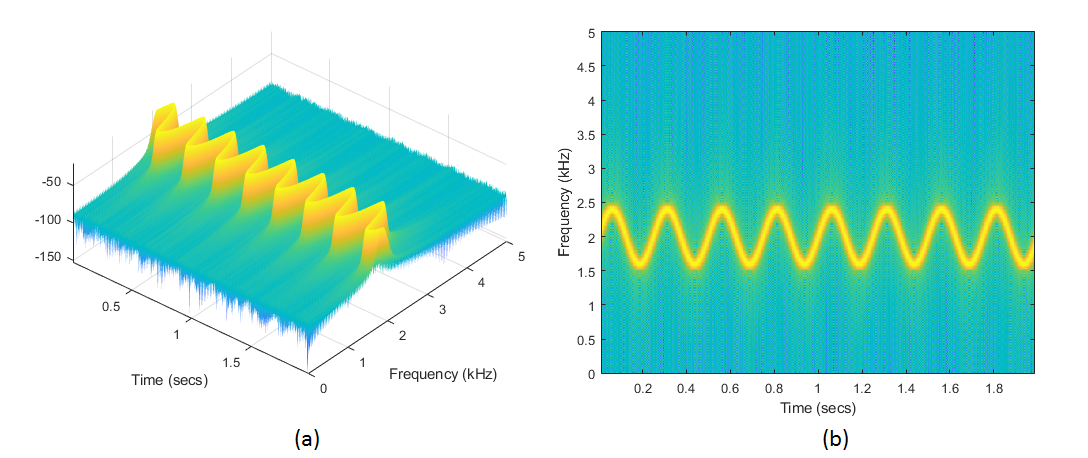
\includegraphics[width=0.9\linewidth]{content/fig/spec_example.png}
    \caption{
    (a) The STFT of a function with varying frequency and, 
    (b) The STFT in (a) visualised as a spectrogram.
    }
    \label{fig:spec_example}
\end{figure}

\subsection{Filterbanks}

Spectrograms are a useful feature for analysing frequency characteristics of a signal, but when it comes to speech in particular, they still contain a lot of unnecessary information. 
Human speech, for instance, falls mainly within 80 Hz and 8 kHz, thus removing the need for very high frequency capturing. 
Even more, the human ear does not distinguish different levels of frequencies equally. 
We are able to distinguish the difference between an 80 Hz signal and a 100 Hz signal far greater than between 3 kHz and 3.1 kHz.

It is this property that gives rise to the Mel-scale. 
The Mel-scale aims The Mel-scale aims to mimic the non-linear human ear perception of sound, by being more discriminative at lower frequencies and less discriminative at higher frequencies. 
We can convert between Hertz ($f$) and Mel ($m$) using the following equations:

\begin{equation}
    m = 2595 \log_{10} (1 + \frac{f}{700})
\end{equation}

\begin{equation}
    f = 700 (10^{m/2595} - 1)
\end{equation}

Filterbanks are calculated by applying triangular filters (usually 40), spaced according to the Mel-scale as shown in Figure~\ref{fig:mel_filters}, over the speech spectrogram. 
This results in a $40\times N$ array, where $N = \frac{\mathrm{time}}{f_s}$, which is much smaller than the previous spectrograms.
These triangular filters can be modelled by the following function:

\begin{equation}
    H_m(k) =
  \begin{cases}
      \hfil 0 & k < f(m - 1) \\
      \dfrac{k - f(m - 1)}{f(m) - f(m - 1)} & f(m - 1) \leq k < f(m) \\
      \hfil {1} & k = f(m) \\
      \dfrac{f(m + 1) - k}{f(m + 1) - f(m)} & f(m) < k \leq f(m + 1) \\
      \hfil {0} & k > f(m - 1) \\
  \end{cases}
\end{equation}

\begin{figure}[h]
    \centering
    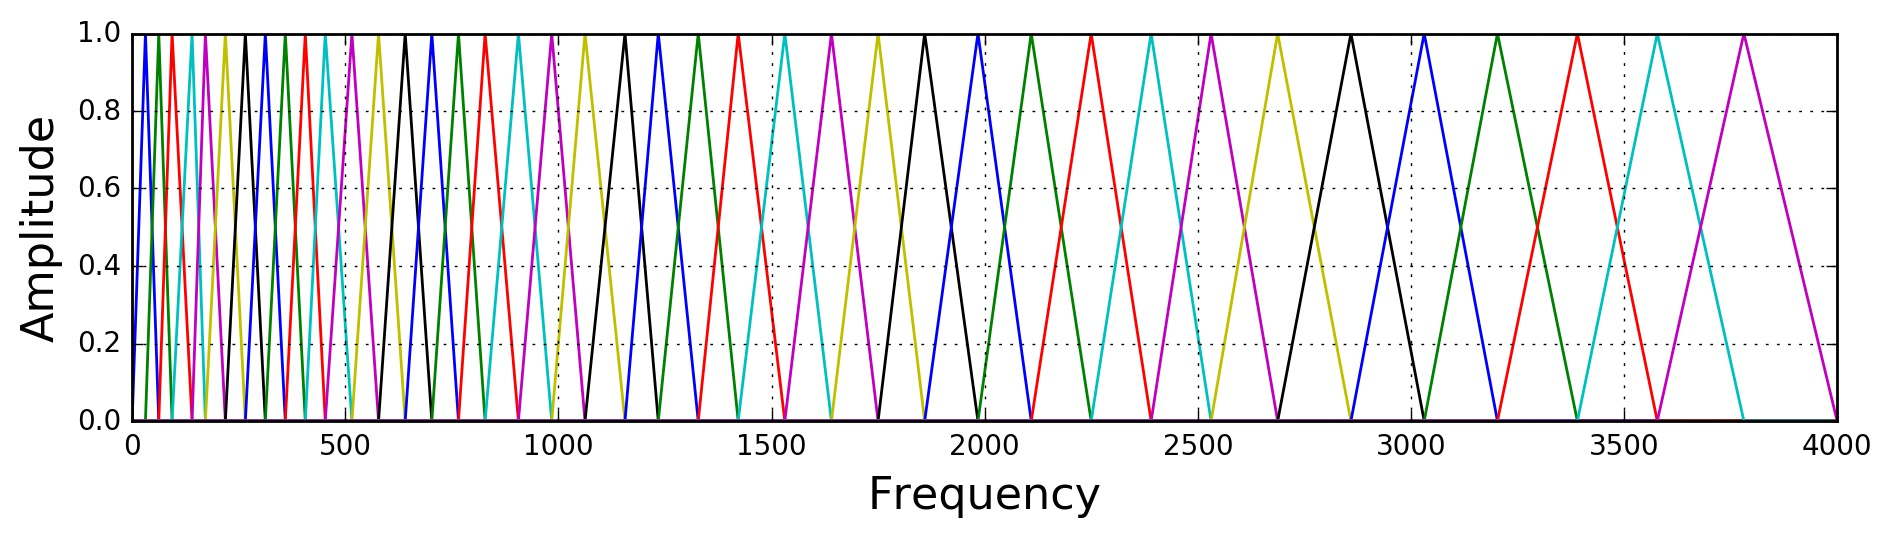
\includegraphics[width=0.9\linewidth]{content/fig/mel_filters.jpg}
    \caption{40 filterbanks on the Mel-scale.}
    \label{fig:mel_filters}
\end{figure}

\subsection{Mel Frequency Cepstral Coefficients (MFCCs)}

Going one step further from filterbanks, Mel Frequency Cepstral Coefficients aim to tackle the highly correlated nature between each filterbank. 
This correlated nature of the filterbanks is because, as can be seen by Figure~\ref{fig:mel_filters}, each filter overlaps with the filters next to it.

To understand how MFCCs aim to tackle this problem, it helps to look at filterbanks as a continuous time signal instead of a discrete frequency spectrum.
The overlapping nature of the filters would then cause small peaks within the resulting signal. 
This can be viewed as high frequency noise on top of the desired signal.

Usually, when we want to remove high frequency noise from a signal, we calculate the FT to transform the signal to the spectral (frequency) domain, then simply remove the higher frequencies. 
When doing calculating the FT of a spectral signal, it is called moving to the cepstral domain, and thus the name, Mel Frequency Cepstral Coefficients.

Instead of calculating the FT of the filterbanks, however, MFCCs are calculated by using the Discrete Cosine Transform (DCT).
The DCT gives a fairly similar result as the DFT, and can be expressed as follows:

\begin{equation}
    X[k] = \mathtt{DCT} \{ x[n] \} = \displaystyle\sum_{n=0}^{N-1} h[n] \cdot \cos\bigg(\displaystyle\frac{\pi}{N}\Big(n+\frac{1}{2}\Big)k\bigg)
\end{equation}

After the DCT for of the filterbanks are calculated, only 12 of the 26 DCT coefficients are kept, removing fast changes in the filterbanks and effectively applying a cepstral LPF on them. 
The energy of each frame is also appended to the bottom of the MFCC to result in a 13 data points per frame.

The MFCC feature vector only describes the spectral envelope of a single frame, but there often lies valuable information in the trajectories of MFCC coefficients over time. 
Therefore, it is common to append the differential (delta) and acceleration (delta-delta) coefficients of the MFCC to the feature vector. 
The delta coefficients are calculated with the following formula:

\begin{equation}
    d_t=\displaystyle\frac{\sum_{n=0}^{N-1} n(c_{t+n}-c_{t-n})}{2\sum_{n=0}^{N-1} n^2}
\end{equation}
where $d_t$ is the delta coefficient and $c_t$ the filterbank value of frame $t$.
$N$ is commonly set to 2. 
The delta-delta coefficients are calculated similarly, except the filterbank values are substituted by the delta coefficients.

Applying all this results in a $26\times N$ array, where $N = \frac{\mathrm{time}}{f_s}$, thus an even smaller feature vector than filterbanks containing more effective information about the speech data.

\section{Convolutional Neural Networks}

In this study we hope to improve upon existing speech feature extraction techniques by using the learned features from image classification CNNs. 
In order to understand how CNNs extract features from images, and automatically learn how to extract the most relevant features, we must first look in to how they work.

\subsection{Convolution}

The main aspect of a CNN is the actual convolutional layers. 
Each layer, as the name suggests, convolves the input it is given with one or multiple filter kernels.
Discrete convolution for one element an input feature $I$ with a $N \times M$ filter kernel $K$ can be defined as follows:

\begin{equation}
    (I \ast K)[i, j] = \displaystyle\sum_{m=0}^{M-1}\displaystyle\sum_{n=0}^{N-1}I[m,n] K[i-m, j-n]
\end{equation}

Performing this operation for every combination of $i$ and $j$ results in a feature map that in essence describes how prominently the feature $K$ appears at each point within $I$.

In practice, CNNs don't actually compute the convolution between two filters, but instead the cross-correlation. 
Since commutativity is not important for most CNNs, it avoids the need of having to flip one of the signals. 
Cross-correlation is very similar to convolution and will be used interchangeably throughout the text.
It can be defined as follows:

\begin{equation}
    (I \ast K)[i, j] = \displaystyle\sum_{m=0}^{M-1}\displaystyle\sum_{n=0}^{N-1}I[m,n] K[i+m, j+n]
\end{equation}

When given an input feature of size $I \times J$, convolved with a filter kernel of $3\times3$, the resultant feature map will be of size $(I-2)\times(J-2)$.
To avoid this, the input feature is often zero padded on each edge with one zero to form an input of size $(I+2)\times(J+2)$, keeping the feature map the same size as the original input.

In neural networks, the act of convolution can be seen as a sparsely connected neural layer. 
Each weight ($h_i$) is connected to a limited amount of input neurons ($x_i$) from the previous layer.
The weight then performs a linear transformation on the input neurons. 
For a one dimensional input and a connection level of 3, this process is visualised in Figure~\ref{fig:cnn_layer}, and can be described as follows:

\begin{equation}
    h_i = \displaystyle\sum_{j=-1}^{1}w_{j}x_{i+j}+b_i
\end{equation}

\begin{figure}[ht]
    \centering
    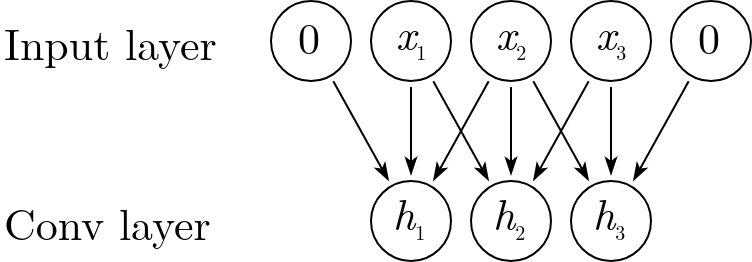
\includegraphics[width=0.5\linewidth]{content/fig/cnn_layer.png}
    \caption{Visualisation of a single convolutional layer.}
    \label{fig:cnn_layer}
\end{figure}

The formula for obtaining the weight is thus equivalent to convolution, with the added benefit of adding a bias $b$ to the final filter result. 

It should also be mentioned that most CNN layers also consist of a ReLU layer, which simply applies an activation function of $f(x)=\mathrm{max}(0,x)$ to the output of the convolutional layer. 
This increases the nonlinear properties of the decision function without affecting the receptive field.\cite{pmlr-v15-glorot11a}

In order to reduce the dimensionality of the feature maps, convolutional neural networks make use of max pooling.
Max pooling simply applies a $N \times N$ filter across its input, outputting only the maximum value within the filter.
The filter is then passed through the entire input, usually with a stride of $N$, reducing the input dimensionality by a factor of $N$.

\subsection{VGG16}

The VGG16 CNN, first proposed by Simonyan et al. \cite{DBLP:journals/corr/SimonyanZ14a}, achieved an image classification accuracy of 92.7\% on the ImageNet database, a data set of more than 14 million images belonging to 1000 different classes, in 2014\cite{ILSVRC15}.
To achieve this accuracy, it employs 13 convolutional layers in total, with 4 max-pooling layers in between to reduce dimensionality.
The full structure can be seen in Figure~\ref{fig:vgg16}.

\begin{figure}[h]
    \centering
    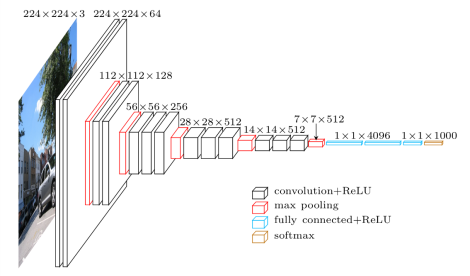
\includegraphics[width=0.6\linewidth]{content/fig/vgg16.png}
    \caption{Macro architecture of VGG16}
    \label{fig:vgg16}
\end{figure}

The VGG16 network makes use of $3\times3$ sized filter kernels with a stride of 1 and a padding of 1 to keep the feature map the same dimensionality as the input.
Max-pooling is performed by a $2\times2$ window with stride 2, effectively halving the first two dimensions of the input.\cite{DBLP:journals/corr/SimonyanZ14a}

For this study, a TensorFlow adaptation of the VGG16 network was used\cite{frossard_2016}.
This model was further adapted to be able to accept differently sized images and added functionality to retrieve the output of each convolutional layer was written.

It should be noted how efficient CNNs can be in extracting features from images.
Where it may seem obvious for humans to design a filter kernel that might detect edges, a CNN can result in kernels that are much less straightforward, but result in far more useful features.
A simple example within the VGG16 network is shown in Figure~\ref{fig:filter_36}, keeping in mind that the first layer of filters are of size $3\times3\times3$, and that the third dimension is displayed as RGB colours.
This shows that a small filter kernel in the first layer of the CNN can already be used to capture features as complex as eyes.

\begin{figure}
    \centering
    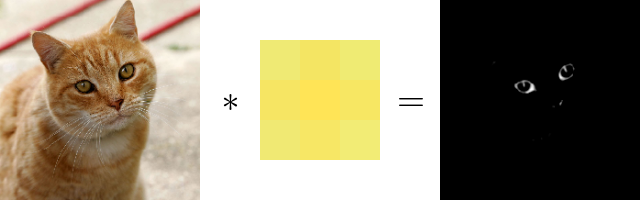
\includegraphics[width=0.6\linewidth]{content/fig/kernel36.png}
    \caption{Example input and output from  kernel 36 of the first convolutional layer in the VGG16 network.}
    \label{fig:filter_36}
\end{figure}

A full list of the first layer of filter kernels can be found in Appendix~\ref{appen:conv1_1}.
Going further down the layers produces even more ambiguous feature maps. 


The ambiguity and general nature of these filter kernels and the feature maps they generate form the basis for employing them as feature extraction techniques for different types of data, such as speech.
\chapter{Feature Evaluation}
\label{chap:evaluation}

Having established the existing feature extraction techniques as well as the new technique proposed by this study, we now look at a method of evaluating these newly extracted features against the existing features proposed by Carlin et al. \cite{DBLP:conf/interspeech/CarlinTJH11}.

The technique consists of using DTW within the same-different speech task for every extracted feature set, then calculating an AP score per feature set using the same-different results.
This process is described fully in the following sections.

\section{Dynamic Time Warping}

Dynamic Time Warping was originally used to normalise for temporal variations between an observed vector time series and a stored template.
It has since been adapted to discover repeated segments in spoken words \cite{DBLP:conf/interspeech/CarlinTJH11}. Given two vectors $\underline{a}$ and $\underline{b}$, we calculate the cosine distance between the vectors as follows:

\begin{equation}
    \mathtt{d}(\underline{a}, \underline{b}) = 1 - \displaystyle\frac{\underline{a} \cdot \underline{b}}{{||\underline{a}||}_2 {||\underline{b}||}_2}
\end{equation}
where ${||\underline{x}||}_2$ is the L2-norm of vector $\underline{x}$.

For a two-dimensional speech feature, such as spectrograms, we calculate the cosine distance for each corresponding frame vector between two words resulting in a distance matrix with structure as follows:

\begin{equation}
    {\mathrm{dist\_mat}}_{m,n} = 
 \begin{bmatrix}
  \mathtt{d}\big(\underline{a}[0], \underline{b}[0]\big) & \mathtt{d}\big(\underline{a}[0], \underline{b}[1]\big) & \cdots & \mathtt{d}\big(\underline{a}[0], \underline{b}[n-1]\big) \\
  \mathtt{d}\big(\underline{a}[1], \underline{b}[0]\big) & \mathtt{d}\big(\underline{a}[1], \underline{b}[1]\big) & \cdots & \mathtt{d}\big(\underline{a}[1], \underline{b}[n-1]\big) \\
  \vdots  & \vdots  & \ddots & \vdots  \\
  \mathtt{d}\big(\underline{a}[m-1], \underline{b}[0]\big) & \mathtt{d}\big(\underline{a}[m-1], \underline{b}[1]\big) & \cdots & \mathtt{d}\big(\underline{a}[m-1], \underline{b}[n-1]\big)
 \end{bmatrix}
\end{equation}
with $\underline{a}$ and $\underline{b}$ the two-dimensional feature vectors of the two words, first dimension the frames and second dimension the frequencies. 

Using this distance matrix, we can calculate a DTW cost matrix by essentially finding the lowest cost path through the distance matrix.
The algorithm to calculate the cost matrix is shown in Algorithm~\ref{alg:dtw}, with only the final value of the cost matrix returned.

\begin{algorithm}
    \caption{Calculating DTW cost matrix}
    \label{alg:dtw}
    \begin{algorithmic}
        \Function{DTWDistance}{$\mathtt{dist\_mat_{m,n}}$}
        \State $\mathtt{cost\_mat} = [0\cdots n, 0\cdots m]$
        \For{$i=1$ to $n+1$}
        \State $\mathtt{cost\_mat}[i, 0] = \infty$
        \EndFor
        \For{$i=1$ to $m+1$}
        \State $\mathtt{cost\_mat}[0, i] = \infty$
        \EndFor
        \For{$i=0$ to $n-1$}
        \For{$j=0$ to $m-1$}
        \State $\mathtt{penalty} = \mathtt{argmin}(\mathtt{cost\_mat}[i, j], \mathtt{cost\_mat}[i, j + 1], \mathtt{cost\_mat}[i+1, j])$
        \State $\mathtt{cost\_mat}[i+1, j+1] = \mathtt{dist\_mat}[i, j] + \mathtt{penalty}$
        \EndFor
        \EndFor
        \State Return $\mathtt{cost\_mat[n, m]}$
        \EndFunction
    \end{algorithmic}
\end{algorithm}

This algorithm is used to define a similarity metric between two spoken word features, with a lower DTW distance expected for the same spoken word, and a higher distance for different words.

It is expected that a better feature extraction technique would more definitively separate similar spoken words from different ones.

To measure the quality of a given feature set, we calculate the DTW distance between each spoken word within the feature set, separating the distances for two of the same words and two different words \cite{kamper_elsner_jansen_goldwater_2015}.

Importantly, iteratively comparing each spoken word to every other spoken word causes the algorithm to be an $O(N^2)$ process, or more precisely it will require $(\frac{N^2-N}{2})$ comparisons, where $N$ is the number of words in the feature set, which for the Buckeye data set consisting of 2\,733 spoken words, requires 3\,733\,278 comparisons per feature set.

\section{Average Precision}

Once we have obtained two lists per feature set, one with DTW distances for similar words and one for different words, we must now determine the separability of the the scores of the two lists.
A possible solution could be to calculate a reliability coefficient for the DTW distances\cite{reliability}, but previous studies have found that skewness in the distributions could lead to instability across different feature sets \cite{DBLP:conf/interspeech/CarlinTJH11}.

Instead, an AP score was calculated by following the method proposed by Carlin et al. \cite{DBLP:conf/interspeech/CarlinTJH11}. To calculate the AP score for a given feature set, we define a threshold $\tau$ for which we assume that for two spoken word vectors, $\underline{a}$ and $\underline{b}$, the two words are the same if $\mathtt{DTW}(\underline{a}, \underline{b}) \leq \tau$. 

For a given value of $\tau$ we are able to calculate two values, namely, the precision and the recall point.
Precision is defined as the percentage of same word pairs whose DTW distance falls below the threshold, and recall is defined as the percentage of different word DTW distances that fall above the threshold.
Sweeping $\tau$ from the minimum DTW distance to the maximum distance for a given feature set allows us to draw a precision-recall curve.
A precision-recall curve for a feature set where the DTW distances are perfectly separated is shown in Figure~\ref{fig:pr-curve}, as well as the spectrograms, filterbanks and MFCCs of the Buckeye data set.

\begin{figure}[h]
    \centering
    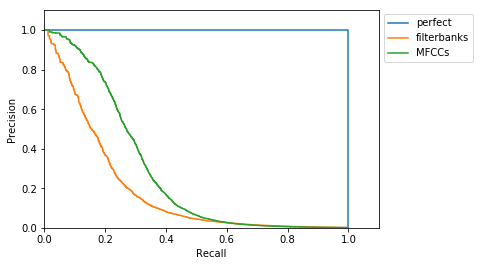
\includegraphics[width=0.8\linewidth]{content/fig/pr_curve.png}
    \caption{Precision-recall curves for a perfectly separable feature set, spectrograms, filterbanks and MFCCs for the Buckeye data set.}
    \label{fig:pr-curve}
\end{figure}

Note that for a perfect precision-recall curve, the area underneath the curve is exactly 1.
For the spectrograms, filterbanks and MFCCs, these areas are 0.02347, 0.189 and 0.2843 respectively.
The area underneath the curve thus acts as a global metric to measure the separability of a given feature set, thus implying a clear improvement in feature quality from filterbanks against spectrograms, and from MFCCs against filterbanks.
It is exactly this metric that we use as our AP score, with a score of 1 denoting a perfect feature set, and the lower the AP score, the generally more difficult it will be for a model to distinguish between words for the given feature set.

This AP score technique has been shown to correlate well with phone recognition error rates \cite{DBLP:conf/interspeech/CarlinTJH11} and has been used in several other unsupervised studies \cite{kamper_elsner_jansen_goldwater_2015}.
\chapter{Experimental Setup}

Various software environments and setups were used during the testing, extracting and evaluation of the features during this study.
We begin by describing the format of the Buckeye data set and VGG16 CNN, followed by a description of the environments in which each step of the feature extraction and evaluation was performed.

\section{Data set}

The Buckeye Corpus of conversational speech contains high-quality recordings from 40 speakers in Columbus OH conversing freely with an interviewer. 
The files are stored in WAV files.
Filterbank and MFCC features for spoken words within this data set were provided by Dr H. Kamper, but since spectrograms would need to be calculated as well, these features were not used. 
Instead, the word label and timestamp for these features were used to develop code to extract spectrograms, filterbanks and MFCCs and stored as Numpy files per feature type, with each individual feature as a numpy array.

The spectrograms were calculated using a Hamming window with a frame length of 25 ms and an overlap of 15 ms.
The log value of each spectrogram was used in order to better normalise the variation in magnitudes.
This resulted in a numpy array of size $201 \times N$, with $N \approx \frac{t}{15\times10^{-3}}$ with $t$ the time in seconds.
Filterbanks and MFCCs were calculated from these spectrograms resulting in $40 \times N$ and $39 \times N$ arrays respectively.

\section{Environments}

The bulk of the code developed for this study was written in Python 3.6, with the exception of the DTW code supplied by H.
Kamper, which was written in Cython, and the Cloud Function used during the feature evaluation, which was written in Node.js v6.
Crucial Libraries included Numpy, TensorFlow, Matplotlib and Scipy.

Though the language of the code was fairly consistent for this study, the different hardware requirements needed to perform the necessary tasks within a reasonable time and without any cost required some creativity, and Google Cloud Platform was used to accomplish many tasks that would otherwise have cost unrealistic amounts of time.

\subsection{Development}

Developing and testing of all functions were first done within a Jupyter Notebook running on a local machine.
This included the development of code to extract the spectrograms, filterbanks and MFCC features from the spoken word WAV files, configuring and alteration of the VGG16 TensorFlow model to support different input sizes as well as output the feature map of each layer, testing and altering of the code needed to perform DTW, the Same-Different Speech task, and to calculate the average precision.
Testing and validation of each function was also performed locally before deployment on a certain GCP service.

\subsection{Google Cloud Platform}

As stated in the sections hereafter, GCP was used for various tasks in this study.
GCP is a cloud computing framework with various SaaS products.
Though these products are charged by use time, GCP offers a 12 month free trial period with \$ 300 credit, with some added limits to the use of certain products.
For the tasks needed in this study, the free trial was found to be sufficient, eliminating any costs.
We discuss the services used in this study, namely GCE, GCS, Cloud Functions and Datalab.

\subsubsection{Google Compute Engine}

GCE is a service that allows users to connect remotely to a VM instance.
The instance types can be tailored specifically to the users needs by specifying the number of CPUs, the size of the memory as well as storage, the OS running on the machine and a bash script to run on start up.
API calls to create, modify and delete VM instances also exist and were used during the feature evaluation task. 

Once the instance is running, users can connect to the console via SSH to run further commands.
During the free trial of GCP, a limit of 8 vCPUs per machine is set, and a maximum of 64 CPUs in use globally.

\subsubsection{Google Cloud Storage}

GCS is a storage service for GCP products.
Files are stored in buckets, with each bucket consisting of a generic folder structure.
GCS has the added benefit of running on GCP servers, gaining read and write speeds >1GB/s from within GCP services.

For this study, all features extracted from the VGG16 network as well as the feature evaluation results were stored on GCS, resulting in $\sim$ 130 GB stored on GCS.

\subsubsection{Cloud Functions}

Cloud Functions allow for event driven server-less applications.
For the tasks in this study, Pub/Sub was used to trigger Node.js Cloud Functions.
Pub/Sub is a event streaming service that reliably transfers data to subscribed services.
Cloud Functions are a useful tool in automating GCP products, as it was used to initiate hundreds of GCE instances simultaneously during the feature evaluation task.
This process is described in detail in Section~\ref{evaluation}.

\subsubsection{Datalab}

Datalab is a service that runs a Jupyter Notebook on a specified GCE instance.
The notebook can then be accessed from a local machine, running any code within it on the GCE instance.
Though it is possible to initialise and run a Jupyter Notebook on a GCE instance normally \cite{gce}, Datalab greatly simplifies the task, as well as allow for a significant bypass of GCP limits, which is further described in Section~\ref{extraction}.

\subsection{Feature Extraction} \label{extraction}

Extracting the speech features from the VGG16 network required that both the spectrogram and filterbanks for each spoken word be pushed through the CNN and the feature map of every filter for every layer be saved.
For the first 7 convolutional layers, this meant $1155\times2$ different feature maps per word.
With a total of 2733 words, this resulted in 6313230 different features.

The problem in performing this task, is that a separate TensorFlow VGG16 graph needed to be initialised for every input feature, given that a TensorFlow graph cannot accept different input sizes.
Since the features were to be stored per convolutional filter and not per spoken word, this resulted in two possible algorithms; 

A loop across the 1155 convolutional filters would be made each time initialising a dictionary for the current filter.
Within this loop, another loop across each of the 2733 words would also be made.
Within this loop, a VGG16 graph would be initialised for the given word, and only the result of a single convolutional filter would be added to the current dictionary of filters, with the key being the current word.
At the end of this loop, the current dictionary of filters would be saved as a numpy file, and the loop would move on to the next convolutional filter.

Though this technique would keep the required memory at a given time to a minimum, the time required to initialise a TensorFlow graph and get the result of a single convolutional filter from it is $\sim$ 1 second.
Having to perform this task 6313230 times would result in an execution time of  over 73 days.
Bearing in mind that this entire process needed to be repeated for both filterbanks and spectrograms, it would result in almost 5 months of processing time just to get the features required for the project

Instead, a loop across each of the 2733 words were run and the result for each of the 1155 filters were calculated per word and stored into separate dictionaries per filter, each saved at the end of the loop.
Though this technique required only 2733 TensorFlow graph initialisations resulting in less than an hour of processing time, it required the full list of 6313230 feature maps to be stored in memory for the duration of the loop.
With an average size of 10.9 kB per feature map, this algorithm would require hardware with a total memory of $\sim$ 70 GB.
Further inefficiencies within Numpy memory usage as well as having to store 2733 tensorflow graphs in memory resulted in a total memory requirement of at least 210 GB.

In order to gain access to such massive memory requirements, GCP's Datalab service was required.
Though the free tier of GCE is limited to the amounts of memory and CPUs available for a single instance (30 GB and 8 vCPUs respectively), when initialised through Datalab, those limits are ignored.
Thus, a Datalab instance was initialised on a n1-highmem-64 GCE instance, resulting in 64 vCPU cores and 416 GB of memory.
The high amount of CPU cores also allowed the algorithm to be calculated simultaneously per spoken word using IPython's BackgroundJobs multithreading library.

The resulting features were then calculated on the Jupyter notebook and the resulting numpy files copied to a GCS bucket, from which it would be available for local usage as well as to any future GCP services.
Features were stored within 2310 numpy archive files, named after the specific convolutional layer and the individual filter kernel from which they were extracted, 1155 were extracted from the log spectrograms and 1155 from the filterbanks. 

For the features extracted from the log spectrograms, the first 2 convolutional layers (conv1\_1 and conv1\_2) resulted in features of the same size as the inputs that they were generated from, thus $201 \times N$ for spectrograms and $40 \times N$ for filterbanks.
Conv2\_1 and conv2\_2 feature maps halved each input axis, and conv3\_1, conv3\_2 and conv3\_3 quartered each input axis.
From Conv3\_1 and onward, some spoken word feature maps started becoming $1\times X$ features, thus making the calculation of an AP score ineffective, thus layers further than conv3\_3 were not used to extract features.

\subsection{Feature Evaluation} \label{evaluation}

In order to evaluate features using the Same-Different Speech task, the DTW distance for each word needed to be calculated and compared to that of every other word, which, for 2733 words, results in 3733278 comparisons.
The time to calculate a single DTW distance on a local machine is on average 4 ms.
Even when optimised to not calculate the same DTW distance twice, this resulted in the time for a single feature type's AP score to take 6 h 15 min.
This task needed to be done for each of the 2310 different features, which if done sequentially would result in 1.6 years of processing time.
Experimentation also showed that multithreading this task per feature did not divide up time linearly, and would still result in a highly unrealistic time frame to complete.

In order to evaluate the features within the given time frame, each feature's AP score would truly need to be computed on a separate machine.
To accomplish this task, A Cloud Function was written that on request, instantiated a 1 CPU core GCE instance with preloaded instructions to download the necessary feature from GCS, run a python script to calculate and save the feature's AP score, copy the resulting file to GCS and then send a message to Pub/Sub message to instantiate another Cloud Function which would in turn destroy the GCE instance.
A script to then call a Cloud Function for each and every feature was then written and run, resulting in 2310 simultaneous GCE instances each computing a single feature's AP score.
Though this would have then only taken 6 h 15 min to complete, an added benefit of GCE (that it ran on Intel Skylake CPUs) resulted in the time to calculate an AP score was brought down to $\sim$ 1 hour.
A visual representation of the work flow is shown in Figure~\ref{fig:workflow}.

\begin{figure}[h]
    \centering
    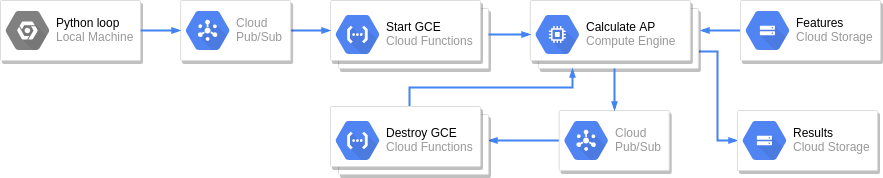
\includegraphics[width=0.9\linewidth]{content/fig/workflow.png}
    \caption{Illustrated GCP work flow to calculate AP score on individual GCE instances.}
    \label{fig:workflow}
\end{figure}

It should be noted that in order to allow for 2310 simultaneous GCE instances, GCP had to be taken out of the free trial period, but billing still continues from the initial \$ 300 credit.
In total, running this algorithm resulted in a cost of \$ 144.50, still staying below the allowed \$ 300 and keeping the tasks for this study without cost.
\chapter{Experiments}
\label{chap:experiments}

Having established our experimental setup and the environments we use, we move on to the experiments themselves. 
Firstly, we establish the benchmark scores for spectrograms, filterbanks and MFCCs.
Thereafter, we evaluate the quality of a single feature map obtained through the VGG16 network on spectrograms, filterbanks and MFCCs as input, as well as examine the qualitative properties of the top feature maps.
Finally, we combine the top features obtained to form a hybrid feature map and evaluate the quality of these combined features.

\section{Benchmark Scores}

In order to compare the quality of our newly acquired features, we need a benchmark score to compare it against. 
As stated in previous chapters, we use the AP scores obtained from the generic spectrograms, filterbanks and MFCCs of the Buckeye Corpus. 
Running the evaluation algorithm described in Chapter~\ref{chap:evaluation} on these features resulted in the AP scores shown in Table~\ref{tbl:benchmarks} and the precision-recall curves shown in Figure~\ref{fig:pr-curve}.

\begin{table}[!ht]
    \mytable
    \caption{Benchmark AP scores for Spectrograms, filterbanks and MFCCs.}
    \begin{tabularx}{0.85\linewidth}{@{}Ll@{}}
        \toprule
        Feature         & AP        \\
        \midrule
        Spectrograms    & $0.02347$ \\
        Filterbanks     & $0.1890$  \\
        MFCCs           & $0.2843$  \\
        \bottomrule
    \end{tabularx}
    \label{tbl:benchmarks}
\end{table}

As expected, spectrograms result in a very low AP score of 0.02347 due to the high variability caused by different speakers, tones, channels and acoustic conditions. 
Filterbanks result in a significant improvement on spectrograms with an AP score of 0.189 due to the reduced impact of frequency ranges that fall outside normal speech. 
MFCCs, with an AP score of 0.2843, further improve on filterbanks by removing much of the spectral noise found within filterbanks as well as added improvement through the use of the delta and delta-delta features.

To gain some insight into how similarity between two of the same words are represented within each of these features, Figure~\ref{fig:cost_matrix} shows the distance matrix between two spoken phrases of the word ``graduate" calculated during Algorithm~\ref{alg:dtw} for spectrograms, filterbanks and MFCCs respectively. 
The DTW algorithm tries to find a minimum cost path from the top left of the cost matrix to the bottom right. 
As can be seen from the distance matrices of the spectrograms and filterbanks, there are clear straight lines and blocks, which is the result of clear differences within the features.
This unnatural distance matrix is an indicator of how ineffectively a feature represents the speech data, with spectrograms being significantly worse than filterbanks.
The distance matrix of the MFCCs, on the other hand, shows a clear natural flow, most likely due to the correlated nature between MFCC frames.
This results in the MFCC being a more effective feature to represent speech data, as is supported by the results in Table~\ref{tbl:benchmarks}.

\begin{figure}[ht]
    \centering
    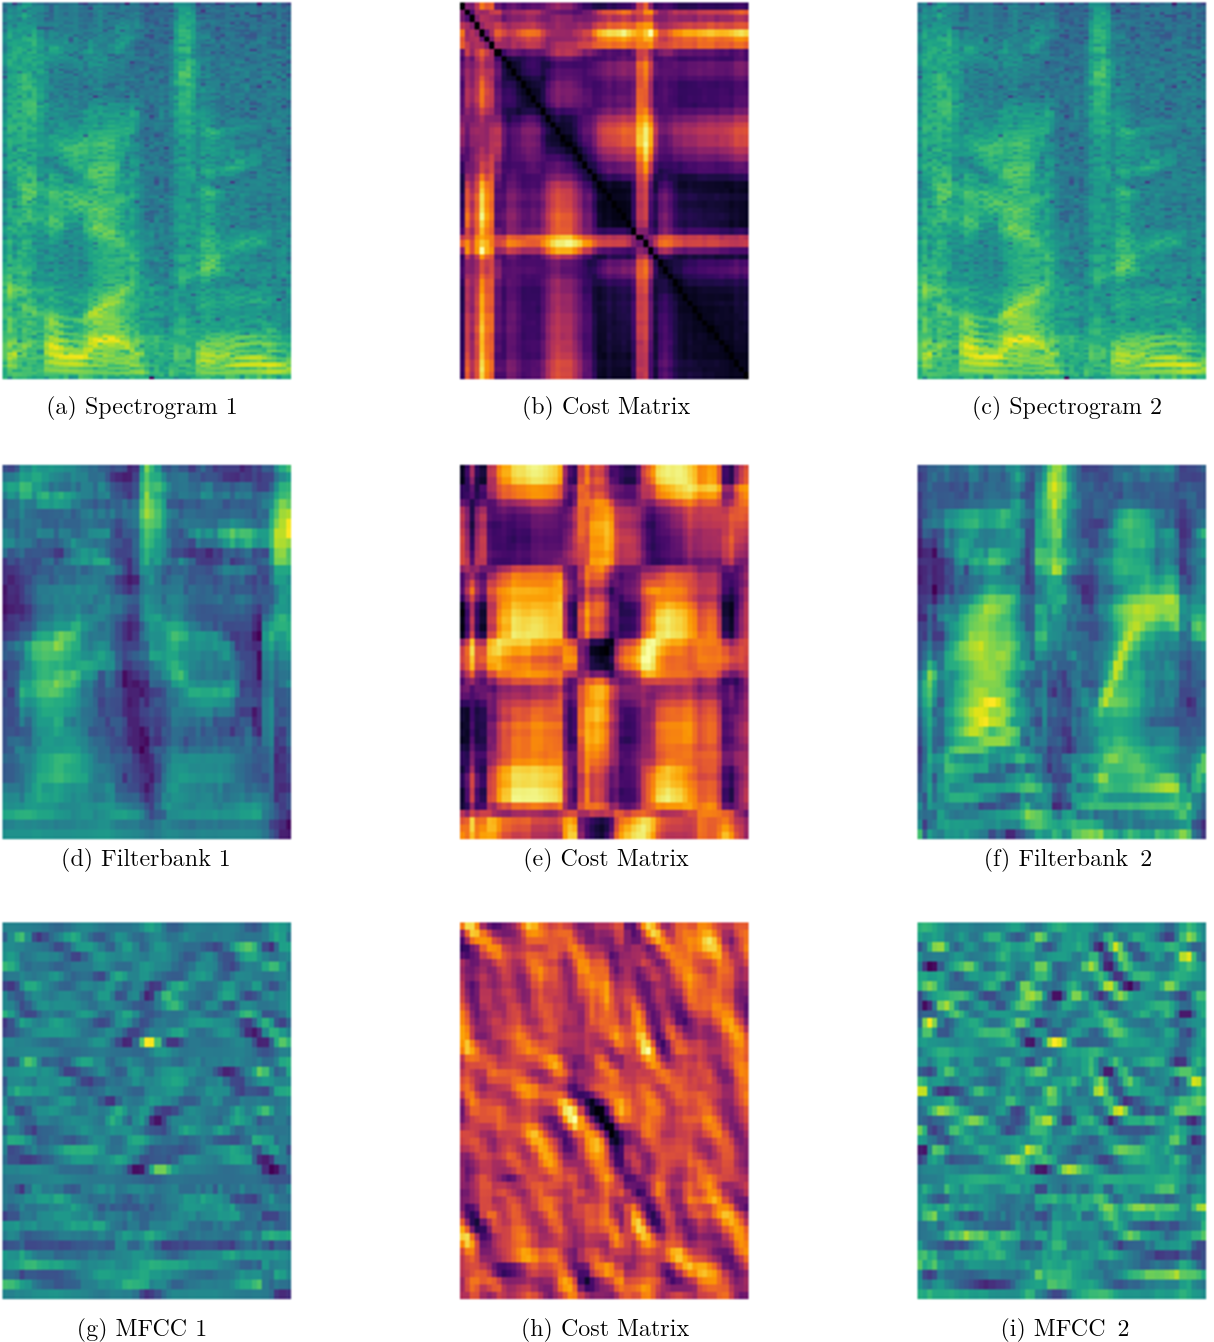
\includegraphics[width=0.9\linewidth]{content/fig/cost_matrices.png}
    \caption{Spectrogram, filterbank and MFCC for two spoken phrases of the word ``graduate" and the distance and cost matrix between each, with lighter colour representing a higher cost.}
    \label{fig:cost_matrix}
\end{figure}

\section{Single Filter Analysis}

Now that our benchmarks have been set, we move on to our first experiment to evaluate the features per individual feature map obtained from the VGG16 network. 
We obtain these features from three input features, namely the spectrograms, filterbanks and MFCCs.
With the features obtained from the spectrogram we at the very least hope to improve our AP score relative to that of the spectrogram benchmark score.
With the features derived from the filterbanks and MFCC we hope to not only improve on the benchmark respective benchmark scores, but also specifically on the MFCC score, thereby improving on existing feature extraction techniques as well as possibly reducing the input vector size.

\subsection{Spectrogram Filters}

When evaluating the feature maps obtained from the spectrograms of the spoken words, we hope to find a feature map that has a more natural distance matrix flow than that of the normal spectrogram, which would ultimately result in a better AP score.
If possible, we hope to find a feature map that outperforms both filterbanks and MFCCs.

The evaluation results, with the top 3 features of each layer shown in Table~\ref{tbl:spectrograms} and all features having an AP score above the spectrogram benchmark shown in Appendix~\ref{appen:ap_scores}, show that there are 167 features that beat the spectrogram benchmark score, with multiple features from every layer in the VGG16 network.
None of the features were able to beat the filterbank or MFCC benchmark, though the top feature, namely \texttt{conv\_2:27}, came within 2\% of the filterbank score, improving upon spectrograms by 691\%.

\begin{table}[!ht]
    \mytable
    \caption{AP scores for the top performing features obtained from spectrograms.}
    \begin{tabularx}{0.85\linewidth}{@{}cLl@{}}
        \toprule
        Rank & Feature        & AP       \\
        \midrule
        11 & 	\texttt{conv1\_1:5} & $0.1106$ \\
        22 & 	\texttt{conv1\_1:16} & $0.0887$ \\
        33 & 	\texttt{conv1\_1:31} & $0.0773$ \\ \hline
        1 & 	\texttt{conv1\_2:27} & $0.1857$ \\
        9 & 	\texttt{conv1\_2:4} & $0.1128$ \\
        15 & 	\texttt{conv1\_2:52} & $0.0955$ \\ \hline
        2 & 	\texttt{conv2\_1:74} & $0.1639$ \\
        6 & 	\texttt{conv2\_1:119} & $0.1196$ \\
        7 & 	\texttt{conv2\_1:90} & $0.1180$ \\ \hline
        3 & 	\texttt{conv2\_2:106} & $0.1613$ \\
        4 & 	\texttt{conv2\_2:6} & $0.1509$ \\
        19 & 	\texttt{conv2\_2:64} & $0.0914$ \\ \hline
        8 & 	\texttt{conv3\_1:119} & $0.1153$ \\
        10 & 	\texttt{conv3\_1:251} & $0.1109$ \\
        12 & 	\texttt{conv3\_1:175} & $0.1066$ \\ \hline
        5 & 	\texttt{conv3\_2:89} & $0.1292$ \\
        16 & 	\texttt{conv3\_2:161} & $0.0950$ \\
        18 & 	\texttt{conv3\_2:143} & $0.0918$ \\ \hline
        20 & 	\texttt{conv3\_3:114} & $0.0910$ \\
        42 & 	\texttt{conv3\_3:88} & $0.0649$ \\
        48 & 	\texttt{conv3\_3:62} & $0.0582$ \\ \hline
        & Benchmark & $0.02347$ \\
        \bottomrule
    \end{tabularx}
    \label{tbl:spectrograms}
\end{table}

Due to these features still being larger vectors than that of filterbanks and MFCCs, it was determined to be an impractical approach to measure combined feature AP scores and thus further increasing the size.
Performing feature extraction on generic spectrograms, though feature quality is improved, can not be a sufficient feature extraction technique when used alone, as it does not reduce feature size enough nor results in a high enough AP score.
Instead, feature extraction was performed on filterbanks and MFCCs in order to obtain at least an equivalent vector size.

\subsection{Filterbank Filters}

For the feature maps obtained from the filterbanks, we hope to find one or more feature maps that beat the AP score of not only the generic filterbank, but also that of the MFCC.
If this feature map could be one obtained from $\mathtt{conv2\_1}$ onward, this would also result in a reduced feature map size whilst improving the feature quality.

When these features were evaluated, the results of which can be seen in Table~\ref{tbl:filterbanks}, it was found that four features outperformed the generic filterbank AP score, with one being from layer $\mathtt{conv2\_1}$, thus halving the input feature and still improving the quality.

It is also interesting to note that none of the features obtained from $\mathtt{conv3\_1}$ were able to beat the benchmark score, suggesting that too small a feature vector may not carry enough information to distinguish words as effectively.

\begin{table}[!ht]
    \mytable
    \caption{AP scores for the top performing features obtained from filterbanks.}
    \begin{tabularx}{0.85\linewidth}{@{}cLl@{}}
        \toprule
        Rank & Feature layer          & AP       \\
        \midrule
        1 & $\mathtt{conv1\_2:9}$     & $0.2363$ \\
        2 & $\mathtt{conv1\_2:26}$    & $0.2287$ \\
        3 & $\mathtt{conv2\_2:27}$    & $0.2148$ \\
        4 & $\mathtt{conv1\_2:53}$    & $0.2124$ \\ \hline
        & Benchmark & $0.1890$ \\
        \bottomrule
    \end{tabularx}
    \label{tbl:filterbanks}
\end{table}
Unfortunately, none of the features obtained were able to beat the MFCC score, but improving upon the generic filterbank score is still a noteworthy achievement, with the top feature improving the AP score by 25\%.
It may also be suggested that the features obtained from layer $\mathtt{conv2\_2:27}$, though not as accurate as MFCCs, could be used for speech recognition where smaller model sizes are required, due to the feature sized being effectively quartered.
We go on to qualitatively examine how these features were able to achieve improved AP scores.

\subsubsection{Qualitative Analysis}

When examining the qualitative properties of the extracted feature maps, shown for the word ``collecting" in Figure~\ref{fig:fbank_features}, there seemed to be a strong tendency within the first, second and fourth feature maps to emphasise frequencies that were gradually rising in time.
This was found to, in most cases, be linked to occurrences where the speaker is switching from a nasal or lateral consonant to a vowel.
This could greatly improve the ability to recognise similar words by more easily recognising similar consonant-to-vowel transitions.

\begin{figure}[ht]
    \centering
    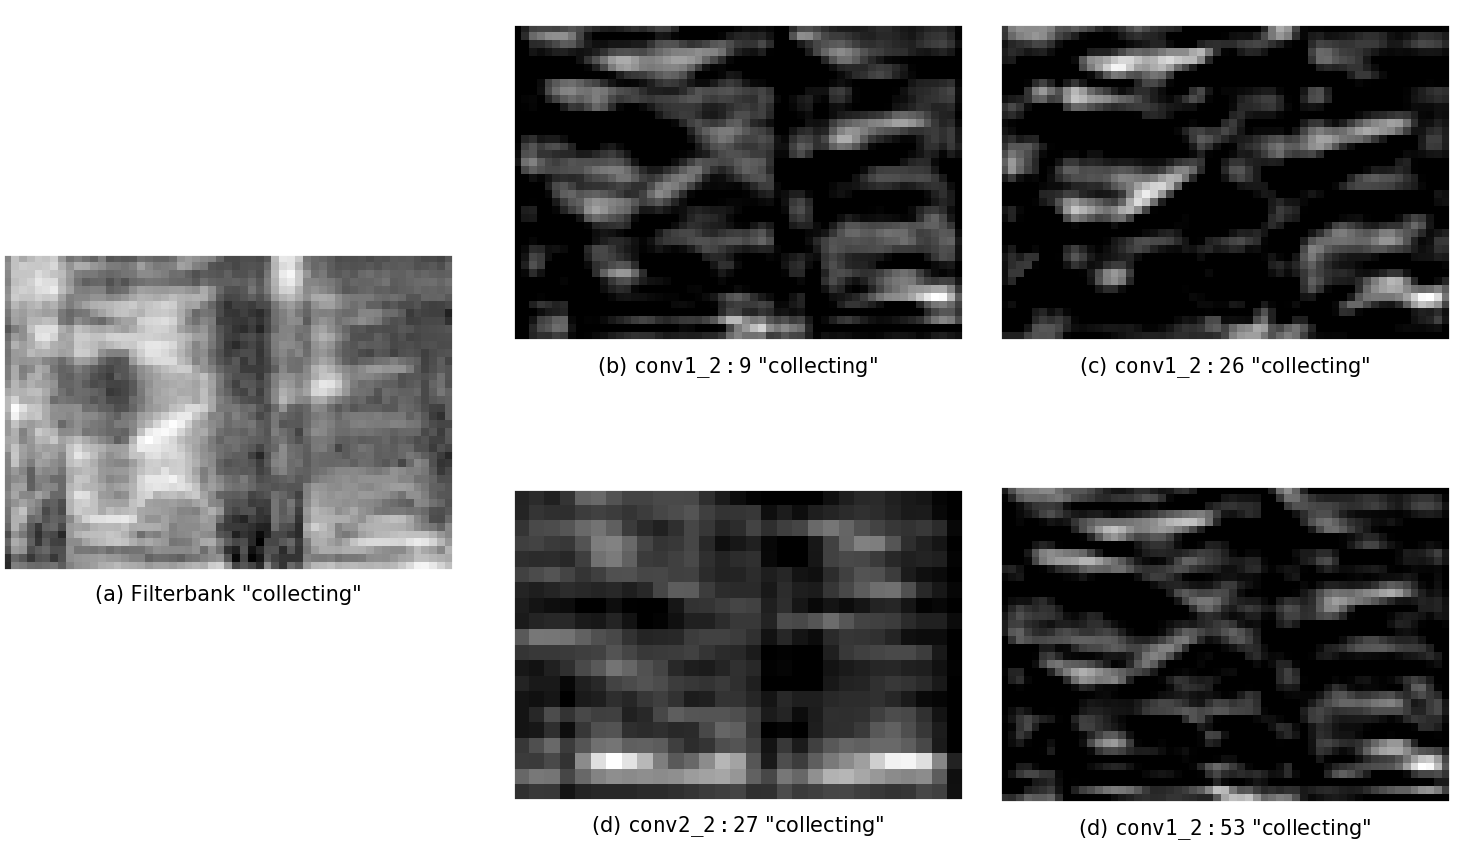
\includegraphics[width=0.5\linewidth]{content/fig/fbank_features.png}
    \caption{The filterbank and corresponding feature maps for the word ``collecting".}
    \label{fig:fbank_features}
\end{figure}

\subsection{MFCC Filters}
\label{chap:mfcc_filters}

For features obtained from the MFCCs, we require that they beat the benchmark score of the MFCC to show any improvement.
If these features could also be obtained from layer $\mathtt{conv2\_1}$ onward, it would also mean that we are able to better represent speech data within a smaller feature vector, greatly improving our feature analysis.

After evaluation, three features were found to beat the MFCC benchmark score, as shown in Table~\ref{tbl:mfccs}. 
Though this does prove our task a success, none of the features were obtained from layer $\mathtt{conv2\_1}$ onward, thus not reducing feature size whilst improving upon quality.

\begin{table}[!ht]
    \mytable
    \caption{AP scores for the top performing features obtained from MFCCs.}
    \begin{tabularx}{0.85\linewidth}{@{}cLl@{}}
        \toprule
        Rank & Feature layer          & AP       \\
        \midrule
        1 & $\mathtt{conv1\_2:17}$    & $0.3064$ \\
        2 & $\mathtt{conv1\_2:37}$    & $0.3007$ \\
        3 & $\mathtt{conv1\_1:9}$     & $0.2960$ \\ \hline
        & Benchmark & $0.2843$ \\
        \bottomrule
    \end{tabularx}
    \label{tbl:mfccs}
\end{table}

In order to try and find a reduced feature input size, we expanded our results to find the top four features obtained from MFCCs from layer $\mathtt{conv2\_1}$ onward that still beat the filterbank benchmark score. These results are shown in Table~\ref{tbl:mfccs2}.
Though these features are of lesser quality than MFCCs, their reduced size may be useful for smaller speech recognition systems that cannot afford such large input vectors.
These features are a quarter the size of the original MFCC input feature, and only reduce the AP score by 16 to 19\%, thus still retaining a fairly high quality.

\begin{table}[!ht]
    \mytable
    \caption{AP scores for the top four performing features obtained from MFCCs from layer $\mathtt{conv2\_1}$ onward.}
    \begin{tabularx}{0.91\linewidth}{@{}cLl@{}}
        \toprule
        Rank & Feature layer          & AP       \\
        \midrule
        1 & $\mathtt{conv2\_1:84}$    & $0.2360$ \\
        2 & $\mathtt{conv2\_1:121}$   & $0.2333$ \\
        3 & $\mathtt{conv2\_1:75}$    & $0.2314$ \\
        4 & $\mathtt{conv2\_1:111}$   & $0.2304$ \\
        \bottomrule
    \end{tabularx}
    \label{tbl:mfccs2}
\end{table}

\subsubsection{Qualitative Analysis}

In order to understand how the top features obtained from the MFCCs improve on its AP score, we look into the qualitative properties of the filters used to obtain these features.

\begin{figure}[h]
    \centering
    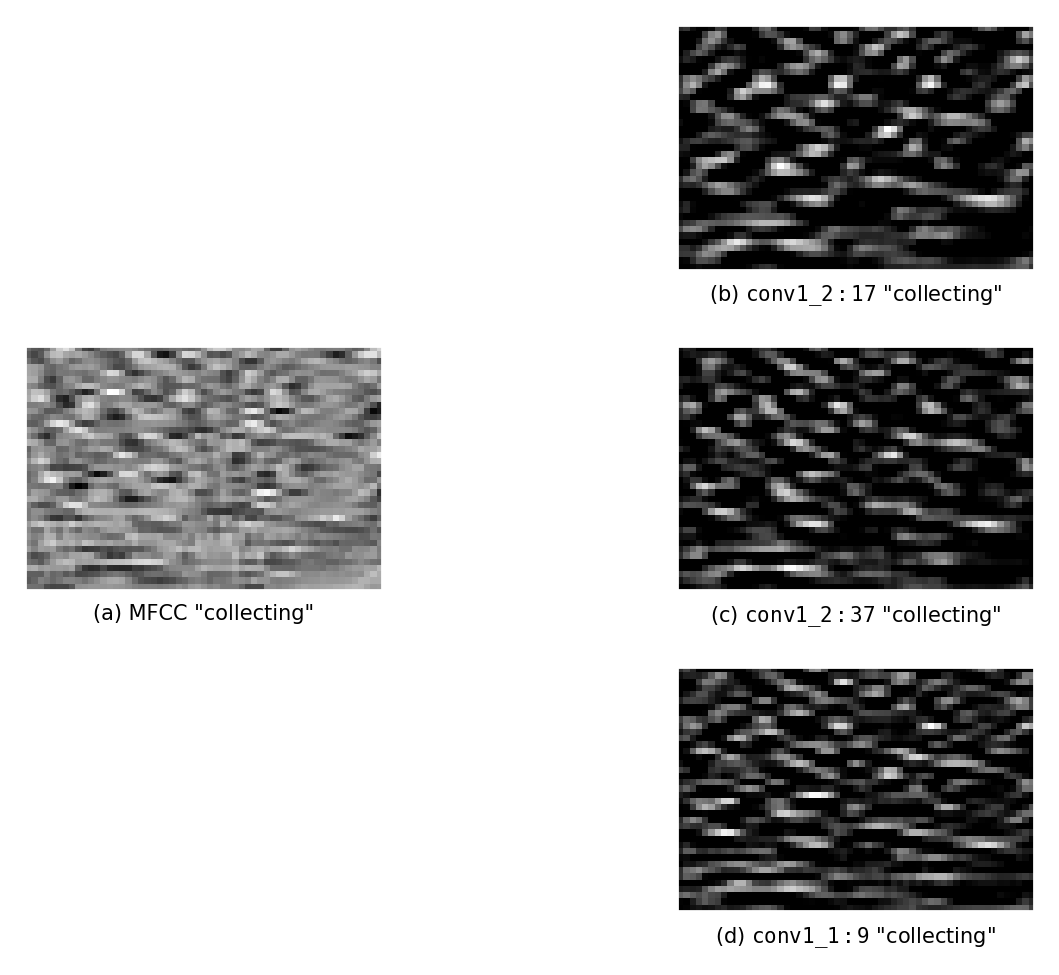
\includegraphics[width=0.5\linewidth]{content/fig/mfcc_features.png}
    \caption{The MFCC and corresponding feature maps for the word ``collecting".}
    \label{fig:mfcc_features}
\end{figure}

Looking at the feature maps extracted for each of these layers for the word ``collecting", shown in Figure~\ref{fig:mfcc_features}, we can see that the top two feature maps are fairly similar.
Upon deeper inspection it was found that these filters act as deeper forms of edge detection, activating over any high spots that are immediately surrounded by fairly low spots.
This has the result of isolating higher volume spots in such a way that it could capture more coherently the parts of speech focused on by humans.
Looking at the third feature map, we can see the filter effect by looking at the filter kernel, shown in Appendix~\ref{appen:conv1_1} ($\mathtt{conv1\_1:9}$).
Keeping in mind that colours are flattened for the speech features, it is clear that the filter kernel also acts as a sort of edge detector, and thus the slight resemblance to the first two feature maps.

\section{Combined Filter Analysis}

In order to try and obtain an even higher AP score whilst retaining feature size, the top four feature maps obtained from the second layer in the VGG16 network ($\mathtt{conv2\_1}$ and $\mathtt{conv2\_2}$) were concatenated to each other to form a single feature map for each of the filterbanks and the MFCCs.
Since the second convolutional layer produces a feature map of size $\frac{N}{2} \times \frac{M}{2}$, with an input feature of size $N \times M$, it in effect quarters the size of the feature.
Thus, concatenating four feature maps from this layer would result in a feature map of size $\frac{N}{2} \times 2M$, which is still the same total size as the original feature vector.
It is the hope that these combined feature maps will each carry different types of information of the spoken word they are derived from, thus acting as a hybrid feature map that performs better than the individual features.

\subsection{Top Filterbank Filters}

For the filterbanks, the top four second layer feature maps are shown in Table~\ref{tbl:fbanks2}.
Though only the top feature actually outperforms filterbanks, it is hoped that each of these features capture a different piece of information of the spoken word and that, if combined, these features will outperform other features.

\begin{table}[!ht]
    \mytable
    \caption{AP scores for the top four features obtained from filterbanks from layer $\mathtt{conv2\_1}$ onward.}
    \begin{tabularx}{0.91\linewidth}{@{}cLl@{}}
        \toprule
        Rank & Feature layer          & AP       \\
        \midrule
        1 & $\mathtt{conv2\_1:27}$    & $0.2148$ \\
        2 & $\mathtt{conv2\_1:15}$   & $0.1754$ \\
        3 & $\mathtt{conv2\_1:62}$    & $0.1479$ \\
        4 & $\mathtt{conv2\_1:1}$   & $0.1479$ \\
        \midrule
        & Combined Features & $0.2622$ \\
        \bottomrule
    \end{tabularx}
    \label{tbl:fbanks2}
\end{table}

An example of this combined filter is shown for the word "collecting" in Figure~\ref{fig:fbank_combined}, which makes it clear how the features are concatenated.

After concatenating all the features, the same AP score algorithm described in Chapter~\ref{chap:evaluation} was run on these features to obtain the AP score shown at the bottom of Table~\ref{tbl:fbanks2}.
Clearly, combining these filters results in a higher AP score than that of the individual filters as well as the benchmark filterbank score.
The combined filters also perform better than any other individual filter obtained from filterbanks, giving merit to the technique of combining top filters.

Unfortunately, the AP score is still 7.8\% lower than that of the MFCC benchmark, but coming this close to the MFCC score certainly provides some evidence that visual feature extraction techniques can be applied to speech data.

\begin{figure}[ht]
    \centering
    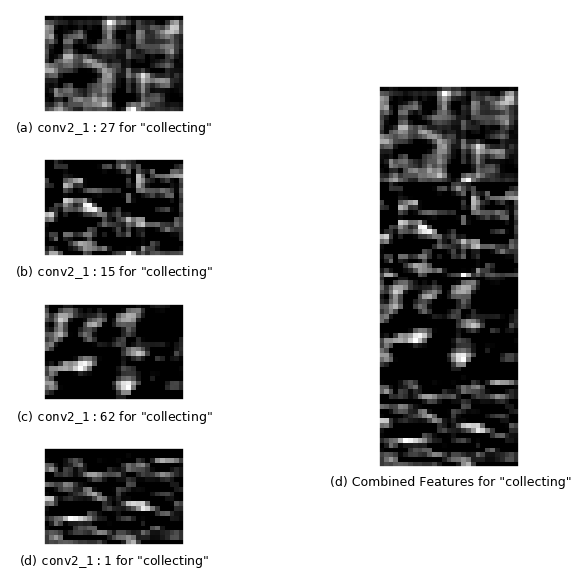
\includegraphics[width=0.5\linewidth]{content/fig/fbankCombined.png}
    \caption{The top four feature maps for the word "collecting" obtained from filterbanks through the second convolutional layer and the combined feature.}
    \label{fig:fbank_combined}
\end{figure}

\subsection{Top MFCC Filters}

Going one step further, we try the same feature combination technique as with filterbanks, combining the top four MFCC feature maps from the second convolutional layer to form a single combined feature.
The AP score of this feature is shown in Table~\ref{tbl:mfcc_combined}.

\begin{table}[!ht]
    \mytable
    \caption{AP score for for the combined feature from the top four features obtained by passing the MFCC through layer $\mathtt{conv2}$.}
    \begin{tabularx}{0.91\linewidth}{@{}Ll@{}}
        \toprule
        Feature layer          & AP       \\
        \midrule
        Combined Feature    & $0.2906$ \\
        \bottomrule
    \end{tabularx}
    \label{tbl:mfcc_combined}
\end{table}

Comparing the AP score to that of the individual features in Table~\ref{tbl:mfccs2} shows that the combined feature yet again outperforms the individual filters as well as the MFCC benchmark.
Unfortunately, it is not able to outperform the top single filter features, falling short by just 5.1\%.

It might be that, as stated in Chapter~\ref{chap:mfcc_filters}, because the properties obtained from the top four features are fairly similar, that combining these specific filters was not as efficient.
There may lie some combination of features that outperform all of the features extracted so far, but due to processing capacity and time limits, this could not be implemented within this study.

\section{Summary of Results}

To summarise the results found in these experiments, Table~\ref{tbl:summarised_results} shows all the top results obtained in a summarised table and the precision-recall curves for all features are shown in Figure~\ref{fig:pr_curves}.
From this Table~\ref{tbl:summarised_results} it is clear that \texttt{conv1\_2:17}, when ran across the MFCC features, is the highest scoring feature, improving the top benchmark score by 7.8\%.

\begin{table}[!ht]
    \mytable
    \caption{Summary of AP Scores for for benchmark features, single filter features per input feature, and combined filter results.}
    \begin{tabularx}{0.91\linewidth}{@{}lcLcl@{}}
        \toprule
        Group       & Rank    & Feature       & Size  & AP Score   \\ \midrule
        Benchmark   & 15 & Spectrograms  & $201 \times N$  & $0.02347$ \\
                    & 11 & Filterbanks   & $40 \times N$  & $0.1890$ \\
                    & 5 & MFCCs         & $39 \times N$  & $0.2843$ \\ \hline
        Spectrogram & 12 & \texttt{conv1\_2:27} & $201 \times N$  & $0.1857$ \\
                    & 13 & \texttt{conv2\_1:74} & $101 \times \frac{N}{2}$  & $0.1639$ \\
                    & 14 & \texttt{conv2\_2:106} & $101 \times \frac{N}{2}$ & $0.1613$ \\ \hline
        Filterbanks & 7 & $\mathtt{conv1\_2:9}$  & $40 \times N$  & $0.2363$ \\
                    & 8 & $\mathtt{conv1\_2:26}$  & $40 \times N$  & $0.2287$ \\
                    & 9 & $\mathtt{conv2\_2:27}$  & $20 \times \frac{N}{2}$  & $0.2148$ \\
                    & 10 & $\mathtt{conv1\_2:53}$  & $40 \times N$  & $0.2124$ \\ \hline
        MFCCs       & \textbf{1} & \texttt{\textbf{conv1\_2:17}}  & $\bm{39 \times N}$  & $\bm{0.3064}$ \\
                    & 2 & $\mathtt{conv1\_2:37}$  & $39 \times N$  & $0.3007$ \\
                    & 3 & $\mathtt{conv1\_1:9}$  & $39 \times N$  & $0.2960$ \\ \hline
        Combined    & 6 & Filterbanks   & $80 \times \frac{N}{2}$  & $0.2622$ \\
                    & 4 & MFCCs         & $78 \times \frac{N}{2}$  & $0.2906$ \\
        \bottomrule
    \end{tabularx}
    \label{tbl:summarised_results}
\end{table}

Some other noteworthy results are the \texttt{conv2\_2:27} feature obtained from the filterbanks, a feature that improves in quality from filterbanks, whilst quartering the feature size.
Another is the combined filterbank feature, providing even better AP scores than any other individual filter obtained from filterbanks.

\begin{figure}[!h]
    \centering
    
\includegraphics[width=0.95\linewidth]{content/fig/pr_all.png}
    \caption{Combined precision-recall curves for all features obtained from (a) spectrograms, (b) filterbanks and (c) MFCCs.}
    \label{fig:pr_curves}
\end{figure}
\graphicspath{{conclusion/fig/}}

\chapter{Summary and Conclusion}
\label{chap:conclusion}

% Bibliography
\bibliography{mybib}

% End matter
\appendix
\chapter{Project Planning Schedule}
\makeatletter\@mkboth{}{Appendix}\makeatother

\begin{table}[!ht]
    \mytable
    \caption{Project goals and planned time frame.}
    \begin{tabularx}{\linewidth}{@{} c  X @{}}
        \toprule
        Time Frame / Date  & \multicolumn{1}{c}{Goal} \\
        \midrule
        12 - 29 June 2018 & Initial research and development of software on existing feature extraction techniques. Set up project outline. \\
        \midrule
        3 - 20 July 2018 & Research and development of TensorFlow and CNN models. \\
        \midrule
        24 July - 5 August 2018 & Initial identification and phrasing of problem and proposed solution. Write abstract. \\
        \midrule
        6 August 2018 & Submit first draft of abstract. \\
        \midrule
        6 - 12 August 2018 & Research Google Cloud Platform and available services. \\
        \midrule
        13 - 31 August 2018 & Develop and test feature extraction software run on Datalab. \\
        \midrule
        17 - 30 September 2018 & Extract features from speech data on Google Datalab. Write initial literature study. Develop and test feature evaluation software. \\
        \midrule
        30 September - 7 October 2018 & Develop high-throughput computing technique for feature evaluation using GCP. Finish literature study on feature extraction and evaluation. \\
        \midrule
        8 October 2018 & Submit first initial report draft. \\
        \midrule
        8 - 21 October 2018 & Run feature evaluation experiments using GCP technique. Ensure software is working correctly and fix any errors. Write experimental setup chapter. \\
        \midrule
        22 - 29 October 2018 & Run any remaining experiments. Finish writing first full draft of report. \\
        \midrule
        30 October 2018 & Submit final draft. \\
        \midrule
        30 October - 4 November 2018 & Amend report and finish any remaining work. Clean up code base. \\
        \midrule
        5 November 2018 & Submit report. \\
        \bottomrule
    \end{tabularx}
    \label{tbl:schedule}
\end{table}

\chapter{Outcomes Compliance}
\makeatletter\@mkboth{}{Appendix}\makeatother

\newcolumntype{R}[1]{>{\centering\let\newline\\\arraybackslash\hspace{0pt}}m{#1}}
\begin{table}[h]
    \mytable
    \caption{The ECSA exit level outcomes and how they were achieved.}
    \begin{tabularx}{\linewidth}{@{} R{4cm} X R{1.3cm} @{}}
        \toprule
        Outcomes & Outcome Description & Pages \\ 
        \midrule
        \textbf{ELO 1: Problem Solving} & The problem of processing all required tasks within a reasonable time was identified and analysed. Various solutions were researched and tested until a suitable solution (GCP services) was identified and implemented. & \textbf{16-18} \\
        \midrule
        \textbf{ELO 2: Application of scientific and engineering knowledge} & Understanding and applying the concepts of spectrograms, filterbanks, MFCCs and convolution required knowledge of mathematics, advanced frequency and cepstral analysis. Skills in computer science and machine learning were necessary for the application and manipulation of CNNs. & \textbf{5-9, 17-18} \\
        \midrule
        \textbf{ELO 3: Engineering Design} & The high-throughput feature evaluation software architecture was designed, developed, analysed, tested and documented. This architecture was developed to be higly extendable and was communicated clearly, the impact and possible uses described. & \textbf{15-18, 31} \\
        \midrule
        \textbf{ELO 4: Investigations, experiments and data analysis} & Various experiments were conducted to evaluate our models, and we make comparisons with previous work by using consistent evaluation metrics and a benchmark dataset. Results are analysed and conclusions are made. & \textbf{20-26, 29-30} \\
        \midrule
        \textbf{ELO 5: Engineering  methods,  skills  and  tools,  including  Information  Technology} & Software languages such as Python, Cython, Node.js were used. Multiple software frameworks and tools such as Jupyter Notebooks, GCE, GCS, Cloud Functions and Datalab were researched and implemented. & \textbf{12, 15-18} \\
        \midrule
        \textbf{ELO 6: Professional and technical communication} & This technical report makes use of appropriate structure, style, and language, and was developed with \LaTeX. & \textbf{1-31} \\
        \midrule
        \textbf{ELO 8: Individual work} & All research, experiments, software development and report writing was done individually.  & \textbf{9-10, 15-16} \\
        \midrule
        \textbf{ELO 9: Independent Learning Ability} & An understanding and high-level competency in TensorFlow CNNs, GCP services and conducting experiments was obtained completely independently. & \textbf{9-10, 15-16} \\
        \bottomrule
    \end{tabularx}
\label{tbl:elo}
\end{table}

\chapter{First Layer Kernels of VGG16}
\makeatletter\@mkboth{}{Appendix}\makeatother
\label{appen:conv1_1}

\begin{figure}[h]
    \centering
    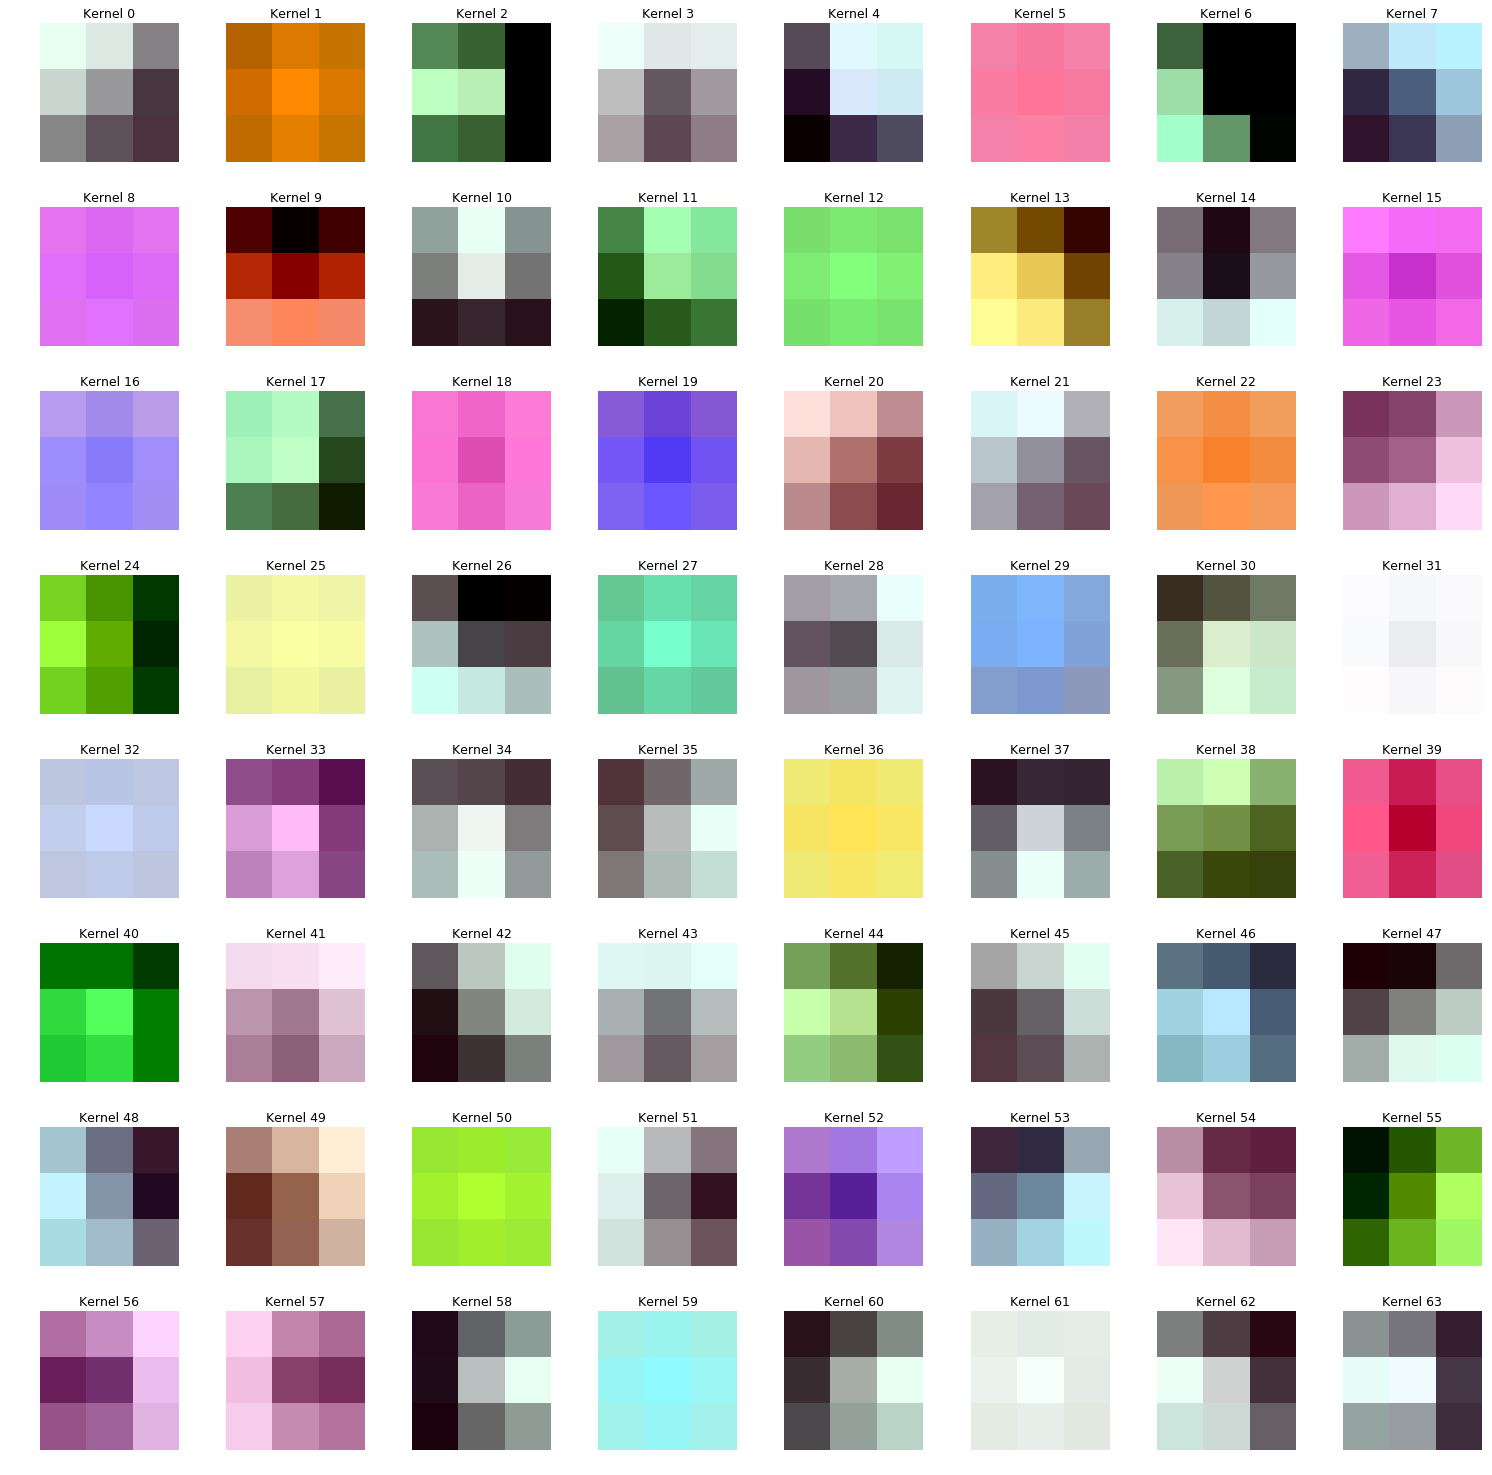
\includegraphics[width=\linewidth]{appendices/fig/conv1_1.png}
    \caption{First layer kernels of VGG16}
    \label{fig:my_label}
\end{figure}

\chapter{Spectrogram features}
\makeatletter\@mkboth{}{Appendix}\makeatother
\label{appen:ap_scores}
\begin{center}
\begin{longtable}{c l l | c l l | c l l }
    \caption{AP scores for the top performing features obtained from spectrograms.}
        \\ \hline
        \# & Feature & AP & \# & Feature & AP & \# & Feature & AP \\ \hline
        1 & \texttt{conv1\_2:27} & $0.186$ & 2 & \texttt{conv2\_1:74} & $0.164$ & 3 & \texttt{conv2\_2:106} & $0.161$ \\
        4 & \texttt{conv2\_2:6} & $0.151$ & 5 & \texttt{conv3\_2:89} & $0.129$ & 6 & \texttt{conv2\_1:119} & $0.120$ \\
        7 & \texttt{conv2\_1:90} & $0.118$ & 8 & \texttt{conv3\_1:119} & $0.115$ & 9 & \texttt{conv1\_2:4} & $0.113$ \\
        10 & \texttt{conv3\_1:251} & $0.111$ & 11 & \texttt{conv1\_1:5} & $0.111$ & 12 & \texttt{conv3\_1:175} & $0.107$ \\
        13 & \texttt{conv3\_1:212} & $0.106$ & 14 & \texttt{conv2\_1:118} & $0.102$ & 15 & \texttt{conv1\_2:52} & $0.095$ \\
        16 & \texttt{conv3\_2:161} & $0.095$ & 17 & \texttt{conv1\_2:2} & $0.092$ & 18 & \texttt{conv3\_2:143} & $0.092$ \\
        19 & \texttt{conv2\_2:64} & $0.091$ & 20 & \texttt{conv3\_3:114} & $0.091$ & 21 & \texttt{conv3\_2:179} & $0.090$ \\
        22 & \texttt{conv1\_1:16} & $0.089$ & 23 & \texttt{conv3\_1:107} & $0.088$ & 24 & \texttt{conv3\_1:57} & $0.087$ \\
        25 & \texttt{conv3\_2:141} & $0.085$ & 26 & \texttt{conv3\_1:247} & $0.084$ & 27 & \texttt{conv2\_1:2} & $0.084$ \\
        28 & \texttt{conv1\_2:25} & $0.083$ & 29 & \texttt{conv2\_2:65} & $0.082$ & 30 & \texttt{conv2\_2:77} & $0.082$ \\
        31 & \texttt{conv3\_1:205} & $0.082$ & 32 & \texttt{conv2\_2:117} & $0.082$ & 33 & \texttt{conv1\_1:31} & $0.077$ \\
        34 & \texttt{conv2\_1:110} & $0.077$ & 35 & \texttt{conv2\_2:90} & $0.076$ & 36 & \texttt{conv2\_2:73} & $0.075$ \\
        37 & \texttt{conv3\_2:50} & $0.074$ & 38 & \texttt{conv1\_2:31} & $0.073$ & 39 & \texttt{conv2\_1:9} & $0.070$ \\
        40 & \texttt{conv2\_1:61} & $0.070$ & 41 & \texttt{conv2\_1:21} & $0.068$ & 42 & \texttt{conv3\_3:88} & $0.065$ \\
        43 & \texttt{conv3\_2:156} & $0.061$ & 44 & \texttt{conv2\_2:127} & $0.061$ & 45 & \texttt{conv2\_2:118} & $0.059$ \\
        46 & \texttt{conv3\_2:35} & $0.059$ & 47 & \texttt{conv2\_1:7} & $0.059$ & 48 & \texttt{conv3\_3:62} & $0.058$ \\
        49 & \texttt{conv2\_2:51} & $0.058$ & 50 & \texttt{conv2\_1:62} & $0.057$ & 51 & \texttt{conv3\_3:249} & $0.057$ \\
        52 & \texttt{conv3\_1:43} & $0.056$ & 53 & \texttt{conv3\_2:129} & $0.056$ & 54 & \texttt{conv2\_1:53} & $0.056$ \\
        55 & \texttt{conv3\_1:38} & $0.055$ & 56 & \texttt{conv2\_1:38} & $0.054$ & 57 & \texttt{conv2\_1:24} & $0.054$ \\
        58 & \texttt{conv3\_2:205} & $0.053$ & 59 & \texttt{conv2\_1:52} & $0.053$ & 60 & \texttt{conv3\_3:125} & $0.052$ \\
        61 & \texttt{conv3\_3:159} & $0.051$ & 62 & \texttt{conv3\_2:109} & $0.051$ & 63 & \texttt{conv2\_1:100} & $0.051$ \\
        64 & \texttt{conv3\_1:201} & $0.050$ & 65 & \texttt{conv3\_1:56} & $0.050$ & 66 & \texttt{conv1\_2:9} & $0.050$ \\
        67 & \texttt{conv2\_1:27} & $0.050$ & 68 & \texttt{conv3\_2:77} & $0.049$ & 69 & \texttt{conv2\_1:50} & $0.049$ \\
        70 & \texttt{conv3\_1:53} & $0.049$ & 71 & \texttt{conv2\_1:5} & $0.049$ & 72 & \texttt{conv3\_1:20} & $0.048$ \\
        73 & \texttt{conv2\_1:71} & $0.048$ & 74 & \texttt{conv2\_2:40} & $0.046$ & 75 & \texttt{conv3\_1:130} & $0.046$ \\
        76 & \texttt{conv3\_1:178} & $0.046$ & 77 & \texttt{conv2\_1:16} & $0.045$ & 78 & \texttt{conv3\_1:27} & $0.043$ \\
        79 & \texttt{conv2\_2:105} & $0.042$ & 80 & \texttt{conv2\_2:94} & $0.042$ & 81 & \texttt{conv2\_1:94} & $0.042$ \\
        82 & \texttt{conv3\_2:37} & $0.042$ & 83 & \texttt{conv1\_2:45} & $0.042$ & 84 & \texttt{conv3\_3:213} & $0.041$ \\
        85 & \texttt{conv2\_1:55} & $0.041$ & 86 & \texttt{conv2\_1:48} & $0.041$ & 87 & \texttt{conv3\_2:63} & $0.040$ \\
        88 & \texttt{conv3\_1:120} & $0.040$ & 89 & \texttt{conv3\_1:16} & $0.040$ & 90 & \texttt{conv2\_1:120} & $0.040$ \\
        91 & \texttt{conv3\_2:255} & $0.040$ & 92 & \texttt{conv3\_1:250} & $0.040$ & 93 & \texttt{conv3\_2:4} & $0.040$ \\
        94 & \texttt{conv1\_2:37} & $0.039$ & 95 & \texttt{conv2\_2:13} & $0.039$ & 96 & \texttt{conv3\_1:198} & $0.039$ \\
        97 & \texttt{conv3\_1:18} & $0.039$ & 98 & \texttt{conv3\_2:216} & $0.039$ & 99 & \texttt{conv3\_2:42} & $0.038$ \\
        100 & \texttt{conv3\_2:31} & $0.038$ & 101 & \texttt{conv2\_1:66} & $0.038$ & 102 & \texttt{conv1\_2:46} & $0.038$ \\
        103 & \texttt{conv3\_2:34} & $0.038$ & 104 & \texttt{conv3\_1:171} & $0.038$ & 105 & \texttt{conv3\_1:245} & $0.037$ \\
        106 & \texttt{conv3\_3:80} & $0.037$ & 107 & \texttt{conv3\_2:210} & $0.036$ & 108 & \texttt{conv2\_2:126} & $0.036$ \\
        109 & \texttt{conv3\_2:187} & $0.035$ & 110 & \texttt{conv3\_3:10} & $0.035$ & 111 & \texttt{conv3\_1:195} & $0.034$ \\
        112 & \texttt{conv3\_1:219} & $0.034$ & 113 & \texttt{conv3\_2:121} & $0.034$ & 114 & \texttt{conv2\_1:73} & $0.034$ \\
        115 & \texttt{conv3\_2:165} & $0.033$ & 116 & \texttt{conv1\_2:34} & $0.033$ & 117 & \texttt{conv3\_1:30} & $0.033$ \\
        118 & \texttt{conv1\_2:13} & $0.033$ & 119 & \texttt{conv2\_1:106} & $0.033$ & 120 & \texttt{conv3\_2:87} & $0.032$ \\
        121 & \texttt{conv3\_2:28} & $0.032$ & 122 & \texttt{conv3\_1:218} & $0.032$ & 123 & \texttt{conv2\_1:96} & $0.032$ \\
        124 & \texttt{conv1\_1:1} & $0.032$ & 125 & \texttt{conv2\_2:4} & $0.031$ & 126 & \texttt{conv3\_3:109} & $0.031$ \\
        127 & \texttt{conv3\_1:72} & $0.031$ & 128 & \texttt{conv3\_2:114} & $0.031$ & 129 & \texttt{conv2\_1:18} & $0.031$ \\
        130 & \texttt{conv2\_1:36} & $0.031$ & 131 & \texttt{conv2\_1:15} & $0.031$ & 132 & \texttt{conv3\_3:234} & $0.030$ \\
        133 & \texttt{conv2\_2:63} & $0.030$ & 134 & \texttt{conv2\_1:49} & $0.030$ & 135 & \texttt{conv3\_1:157} & $0.030$ \\
        136 & \texttt{conv3\_2:48} & $0.030$ & 137 & \texttt{conv3\_2:195} & $0.029$ & 138 & \texttt{conv1\_2:60} & $0.029$ \\
        139 & \texttt{conv1\_2:26} & $0.029$ & 140 & \texttt{conv2\_1:112} & $0.029$ & 141 & \texttt{conv3\_2:153} & $0.028$ \\
        142 & \texttt{conv3\_2:144} & $0.028$ & 143 & \texttt{conv3\_2:5} & $0.028$ & 144 & \texttt{conv3\_2:196} & $0.028$ \\
        145 & \texttt{conv3\_2:167} & $0.028$ & 146 & \texttt{conv3\_3:162} & $0.028$ & 147 & \texttt{conv2\_2:11} & $0.027$ \\
        148 & \texttt{conv3\_2:94} & $0.027$ & 149 & \texttt{conv3\_1:172} & $0.027$ & 150 & \texttt{conv1\_2:53} & $0.027$ \\
        151 & \texttt{conv2\_2:102} & $0.026$ & 152 & \texttt{conv1\_2:17} & $0.026$ & 153 & \texttt{conv3\_2:68} & $0.026$ \\
        154 & \texttt{conv2\_2:7} & $0.026$ & 155 & \texttt{conv3\_2:46} & $0.025$ & 156 & \texttt{conv2\_1:35} & $0.025$ \\
        157 & \texttt{conv3\_2:227} & $0.025$ & 158 & \texttt{conv3\_2:39} & $0.025$ & 159 & \texttt{conv3\_3:178} & $0.025$ \\
        160 & \texttt{conv3\_2:140} & $0.025$ & 161 & \texttt{conv3\_2:248} & $0.025$ & 162 & \texttt{conv3\_1:246} & $0.025$ \\
        163 & \texttt{conv1\_1:36} & $0.025$ & 164 & \texttt{conv3\_2:240} & $0.024$ & 165 & \texttt{conv3\_2:208} & $0.024$ \\
        \hline
    \label{tbl:spectrograms_full}
\end{longtable}
\end{center}



\end{document}

